\documentclass[sigconf]{acmart}

%\usepackage{booktabs} % For formal tables
\usepackage{bm}
\usepackage{multirow}
\usepackage{xspace}
\usepackage[tight,footnotesize]{subfigure}

\newtheorem{myDef}{Definition}
\newtheorem{exmp}{Example}
\newcommand{\paratitle}[1]{\vspace{1.5ex}\noindent\textbf{#1}}
\newcommand{\ie}{\emph{i.e.,}\xspace}
\newcommand{\aka}{\emph{a.k.a.,}\xspace}
\newcommand{\eg}{\emph{e.g.,}\xspace}
\newcommand{\etal}{\emph{et al.}\xspace}
\newcommand{\wrt}{\emph{w.r.t.}\xspace}
\newcommand{\ignore}[1]{}

\copyrightyear{2018} 
\acmYear{2018} 
\setcopyright{acmcopyright}
\acmConference[KDD 2018]{24th ACM SIGKDD International Conference on Knowledge Discovery \& Data Mining}{August 19--23, 2018}{London, United Kingdom}
\acmBooktitle{KDD 2018: 24th ACM SIGKDD International Conference on Knowledge Discovery \& Data Mining, August 19--23, 2018, London, United Kingdom}
\acmPrice{15.00}
\acmDOI{10.1145/3219819.3219965}
\acmISBN{978-1-4503-5552-0/18/08} 
\fancyhead{}

\author{Binbin Hu, Chuan Shi*}
%\authornote{Corresponding author}
\affiliation{%
  \institution{Beijing University of Posts and Telecommunications, Beijing, China}
}
\email{{hubinbin, shichuan}@bupt.edu.cn}

\author{Wayne Xin Zhao}
\authornote{Corresponding author}
\affiliation{%
  \institution{School of Information, Renmin University of China, Beijing, China}
}
\email{batmanfly@gmail.com}

\author{Philip S. Yu}
\authornote{Philip S. Yu is also with the Institute for Data Science, Tsinghua University, Beijing, China.}
\affiliation{%
  \institution{University of Illinois at Chicago}
  \city{IL}
  \country{USA}
}
\email{psyu@cs.uic.edu}


%\author{Binbin Hu}
%\affiliation{%
%  \institution{Beijing University of Posts and Telecommunications}
%  \city{Beijing}
%  \state{China}
%}
%\email{hubinbin@bupt.edu.cn}

%\author{Chuan Shi*}
%\authornote{Chuan Shi is the Corresponding author}
%\affiliation{%
%  \institution{Beijing University of Posts and Telecommunications}
%  \city{Beijing}
%  \state{China}
%}
%\email{shichuan@bupt.edu.cn}

%\author{Wayne Xin Zhao}
%\authornote{Corresponding author}
%\affiliation{%
%  \institution{School of Information, Renmin University of China}
%\city{Beijing}
%\country{China}
%}
%\email{batmanfly@gmail.com}

%\author{Philip S. Yu}
%\authornote{Philip S. Yu is also with the Institute for Data Science, Tsinghua University, Beijing, China.}
%\affiliation{%
%  \institution{University of Illinois at Chicago}
%  \city{IL}
%  \country{USA}
%}
%\email{psyu@cs.uic.edu}


\begin{document}
\title{Leveraging Meta-path based Context for Top-$N$ Recommendation with A Neural Co-Attention Model}

\begin{abstract}
Heterogeneous information network (HIN) has  been widely adopted in recommender systems due to its excellence in modeling complex context information.  
Although existing HIN based recommendation methods have achieved performance improvement to some extent, they have two major shortcomings. First, these models seldom learn an explicit representation for path or meta-path in the recommendation task. Second, they do not consider the mutual effect between the meta-path and the involved user-item pair in an interaction. 
To address these issues, we develop a novel deep neural network with the co-attention mechanism for leveraging rich meta-path based context for top-$N$ recommendation. 
We elaborately design a three-way neural interaction model by explicitly incorporating meta-path based context.
 To construct the meta-path based context, we propose to use a priority based sampling technique to select high-quality path instances.
 Our model is able to learn effective representations for users, items and meta-path based context for implementing a powerful interaction function.
The co-attention mechanism  improves the representations for  meta-path based context, users and items in a mutual enhancement way. 
Extensive experiments on three real-world datasets have demonstrated the effectiveness of the proposed model.
In particular, the proposed model performs well in the cold-start scenario and has potentially good interpretability for the recommendation results.
\end{abstract}

\begin{CCSXML}
<ccs2012>
<concept>
<concept_id>10002951.10003227.10003351.10003269</concept_id>
<concept_desc>Information systems~Collaborative filtering</concept_desc>
<concept_significance>500</concept_significance>
</concept>
<concept>
<concept_id>10010520.10010521.10010542.10010546</concept_id>
<concept_desc>Computer systems organization~Heterogeneous (hybrid) systems</concept_desc>
<concept_significance>500</concept_significance>
</concept>
</ccs2012>
\end{CCSXML}

\ccsdesc[500]{Information systems~Collaborative filtering}
\ccsdesc[500]{Computer systems organization~Heterogeneous (hybrid) systems}

\keywords{Recommender System; Heterogeneous Information Network; Deep Learning; Attention Mechanism}

\maketitle

\section{Introduction}
In the era of information overload, recommender systems play a pivotal role in various online services, which aim to match user interests with resource items~\cite{sarwar2001item}.
Classic recommendation methods, \eg matrix factorization~\cite{koren2015advances}, mainly model users' preference towards items using historical user-item interaction records. Nowadays, various kinds of auxiliary data become increasingly available in online services. Many methods further propose to leverage these context information for improving recommendation performance~\cite{ronen2016recommendations,adomavicius2015context}.
Due to the heterogeneity and complexity of auxiliary data, it is still challenging to effectively utilize such context information in recommender systems.


%With the rapid growth of Web techniques, various kinds of auxiliary data become available in recommender systems. Although auxiliary data is likely to contain useful information for recommendation~\cite{}, it is difficult  to effectively utilize these heterogeneous and complex information in recommender systems.

%Recommender systems mainly aim to model users's preference towards items based on the historical user-item interaction records (\eg user-item rating matrix), known as collaborative filtering~\cite{he2016fast}. In this setting, matrix factorization (MF) remains as one of the most popular collaborative filtering techniques, which simply models the interaction between users and items as the inner product of their latent factors. Despite the effectiveness of MF for recommendation, it may be not sufficient to capture the complex structure of user interaction data via the simple multiplication of latent features linearly.

As a promising direction, \emph{heterogeneous information network} (HIN), consisting of multiple types of nodes and links, has been proposed as a general information modeling method~\cite{sun2011pathsim,shi2017survey}.
Since HIN is flexible to characterize various kinds of heterogenous data, it has been adopted
  in recommender systems to model rich auxiliary data~\cite{zhao2017meta,yu2014personalized}.
In particular,  \emph{meta-path},  a relation sequence connecting object pairs in HIN, is widely used to extract structural features that capture relevant  semantics  for recommendation~\cite{sun2011pathsim}.
We present an example for movie recommendation characterized by HIN in Fig.~\ref{fig-framework-intro}(a).
Roughly speaking, existing HIN based recommendation methods can be categorized into two types.
The first type leverages path based semantic relatedness over HIN as \emph{direct features} for recommendation relevance~\cite{feng2012incorporating,yu2014personalized,shi2015semantic}.  %These methods usually utilize meta-paths to extract or characterize structural features of object pairs, which is mainly used for similarity measurement.
As a comparison, the second type performs some transformation  on path based similarities (\eg matrix factorization on the path based similarity matrix) for learning effective \emph{transformed features}, which are subsequently used to enhance original user or item representations in the recommendation methods~\cite{yu2014personalized,zhao2017meta}.
These two types of methods both extract meta-path based features for improving the characterization of two-way user-item interaction, as illustrated in Fig.~\ref{fig-framework-intro}(b).
%The two types of methods correspond to the full line and dot dash line respectively in Fig.~\ref{fig-framework-intro}(b).

%Existing methods Recently, a number of methods have been proposed to exploit the rich relations in HIN, which can be roughly categorized  into two types. (1) One type of methods learn the latent factors (or embeddings) of users and items for recommendation (see the full line in Figure 1(b))\cite{yu2013collaborative,luo2014hete,shi2016integrating}. These methods usually factorize a matrix of users and items, which is the interaction matrix (e.g., rating matrix) or relation matrix extracted from meta paths, under the matrix factorization framework. Recently, some deep neural network are also been employed to learn refined latent factors \cite{he2017neural,tay2018latent}. (2) The other type of methods leverage path based semantic relatedness between users and items over HINs for recommendation (see the dot dash line in Figure 1(b))\cite{feng2012incorporating,yu2013collaborative,yu2014personalized,shi2015semantic,shi2016integrating}.  These methods usually utilize meta paths to extract or measure structure features of object pairs (e.g., similarity measure), which can also been seen as a kind of embedding information. With the surge of network embedding, path based node embedding in HIN can also been used for recommendation \cite{dong2017meta-path2vec,fu2017hin2vec}.


%Under the HIN-based representation, the recommendation problem can be considered as a similarity search task over the HIN~\cite{sun2011pathsim}.
%Such a recommendation setting is called as \emph{HIN-based recommendation}~\cite{yu2013collaborative}.
%HIN-based recommendation has received much attention in the literature~\cite{feng2012incorporating,yu2013collaborative,yu2014personalized,shi2015semantic,shi2016integrating}.
% The basic idea of most existing HIN-based recommendation methods is to leverage path based semantic relatedness between users and items over HINs, \eg meta-path based similarities,
% for recommendation.

%Recently, due to powerful representations abilities~\cite{hinton2006reducing}, deep learning has achieved substantial successful in various areas including computer vision, neural language process and speech recognition~\cite{collobert2008unified,he2016deep,hong2015understanding}. A few efforts have also been made to apply deep learning to model users' complex bsehaviors in recommender systems, such as neural rating prediction~\cite{salakhutdinov2007restricted}, auto-encoder based recommendation~\cite{wang2015collaborative} and neural collaborative filtering~\cite{he2017neural}.

Although the above methods have achieved performance improvement to some extent,
there are two major shortcomings with existing HIN based methods.
First, they do not learn an explicit representation for path or meta-path in the recommendation method, or the learned representations are not tailored for the recommendation task.  %They typically hold the assumption that path-based similarities indicate relevance evidence for recommendation, which may not be true in all the cases.
Second, they still characterize two-way user-item interactions,  and seldom consider the mutual effect between the meta-path and the involved user-item pair in an interaction.
Without considering the above two aspects, path based features  may not be optimal for  recommendation, and lack direct explanations of why they work or not.
In addition,  existing HIN based recommendation~\cite{shi2017heterogeneous,zhao2017meta} methods mainly focus on the task of rating prediction, while we may only have  implicit feedback available  in practice.
 %user, item and meta-path.  Without an explicit path representation for the recommendation task,


%in which the path-based information has been

%First, the similarities or latent features derived from meta-paths  are usually learned independent of the recommendation task, which makes it difficult to guarantee the performance improvement in complicated recommendation scenarios. Previous methods typically hold the assumption that path-based similarities indicate direct relevance evidence for recommendation. Such an assumption is too strict for a flexible and effective recommendation method.
%Second, they still characterize two-way user-item interactions,  and don't learn explicit representations for paths or meta-paths in the recommendation method.
%The derived path based features are usually transformed into auxiliary representations for  improving original user or item representations. In this way, the learned path-based features are either user- or item-specific, but not interaction-specific. Such an approach is difficult to fully utilize useful information from meta-paths, and can't adapt to varying interactions in recommendation. For example, even a same path instance from some meta-path is likely to convey different semantics for different interactions.

%, since each user-item interaction may depend on different meta-path context.
%the derived path based features (\ie the second type) is not explicitly integrated into the interaction and . Intuitively, even a same meta-path can convey different relevant semantics for different users in varying interactions.

%First, these methods still follow traditional recommendation way which characterises
%(1) First, although embedding of users and items have been extensively studied, the embedding of the $\langle$user, item$\rangle$ pair seldom be exploited, which is also important for recommendation. In HIN, a $\langle$user, item$\rangle$ pair connected by many meta paths contain rich  structure and semantic information, which is useful for recommendation. Although, in the past two years, some HIN embedding methods \cite{dong2017meta-path2vec,fu2017hin2vec} have been proposed,  they focus on node embeddings, rather than node pair embedding. Although proximity embedding \cite{liu2017semantic}  has been proposed for a pair embedding, its blind random walk strategy may lose much semantic information. (2) In addition, the correlation of object embedding and pair embedding have never been exploited until now. A $\langle$user, item$\rangle$ pair consists of a user and an item, so their embedding should be correlated. Unfortunately, pervious methods have never utilized their correlations. (3) Last but not the least, previous HIN-based recommendations focus on the rating prediction task. It may be not really useful in real applications, since users usually care about not predicted scores, but ranking list.

%meta-path based similarities rely on explicit path reachability,HIN-based
%and may not be reliable to be used for recommendation when
%path connections are sparse or noisy.
%It is likely that some links in HINs are accidentally formed which do not convey meaningful semantics.
%Second, meta-path based similarities mainly characterize semantic relations defined over HINs, and may not be directly applicable to
%recommender systems.
%It is likely that the derived path based similarities have no explicit impact on the recommendation performance in some cases.
%Existing methods mainly learn a linear weighting mechanism to combine the path based similarities~\cite{shi2016integrating} or latent factors~\cite{yu2013collaborative}, which cannot learn the complicated mapping mechanism of HIN information for recommendation.
%The two problems essentially reflect two fundamental i<ssues for HIN-based recommendation, namely effective information extraction and exploitation based on HINs for recommendation. Moreover, traditional recommendation methods tend to merely model users and items, while ignore the relation between users and items. Hence, these methods would like to lose many information and harm the recommendation performance.

\begin{figure}
  \centering
  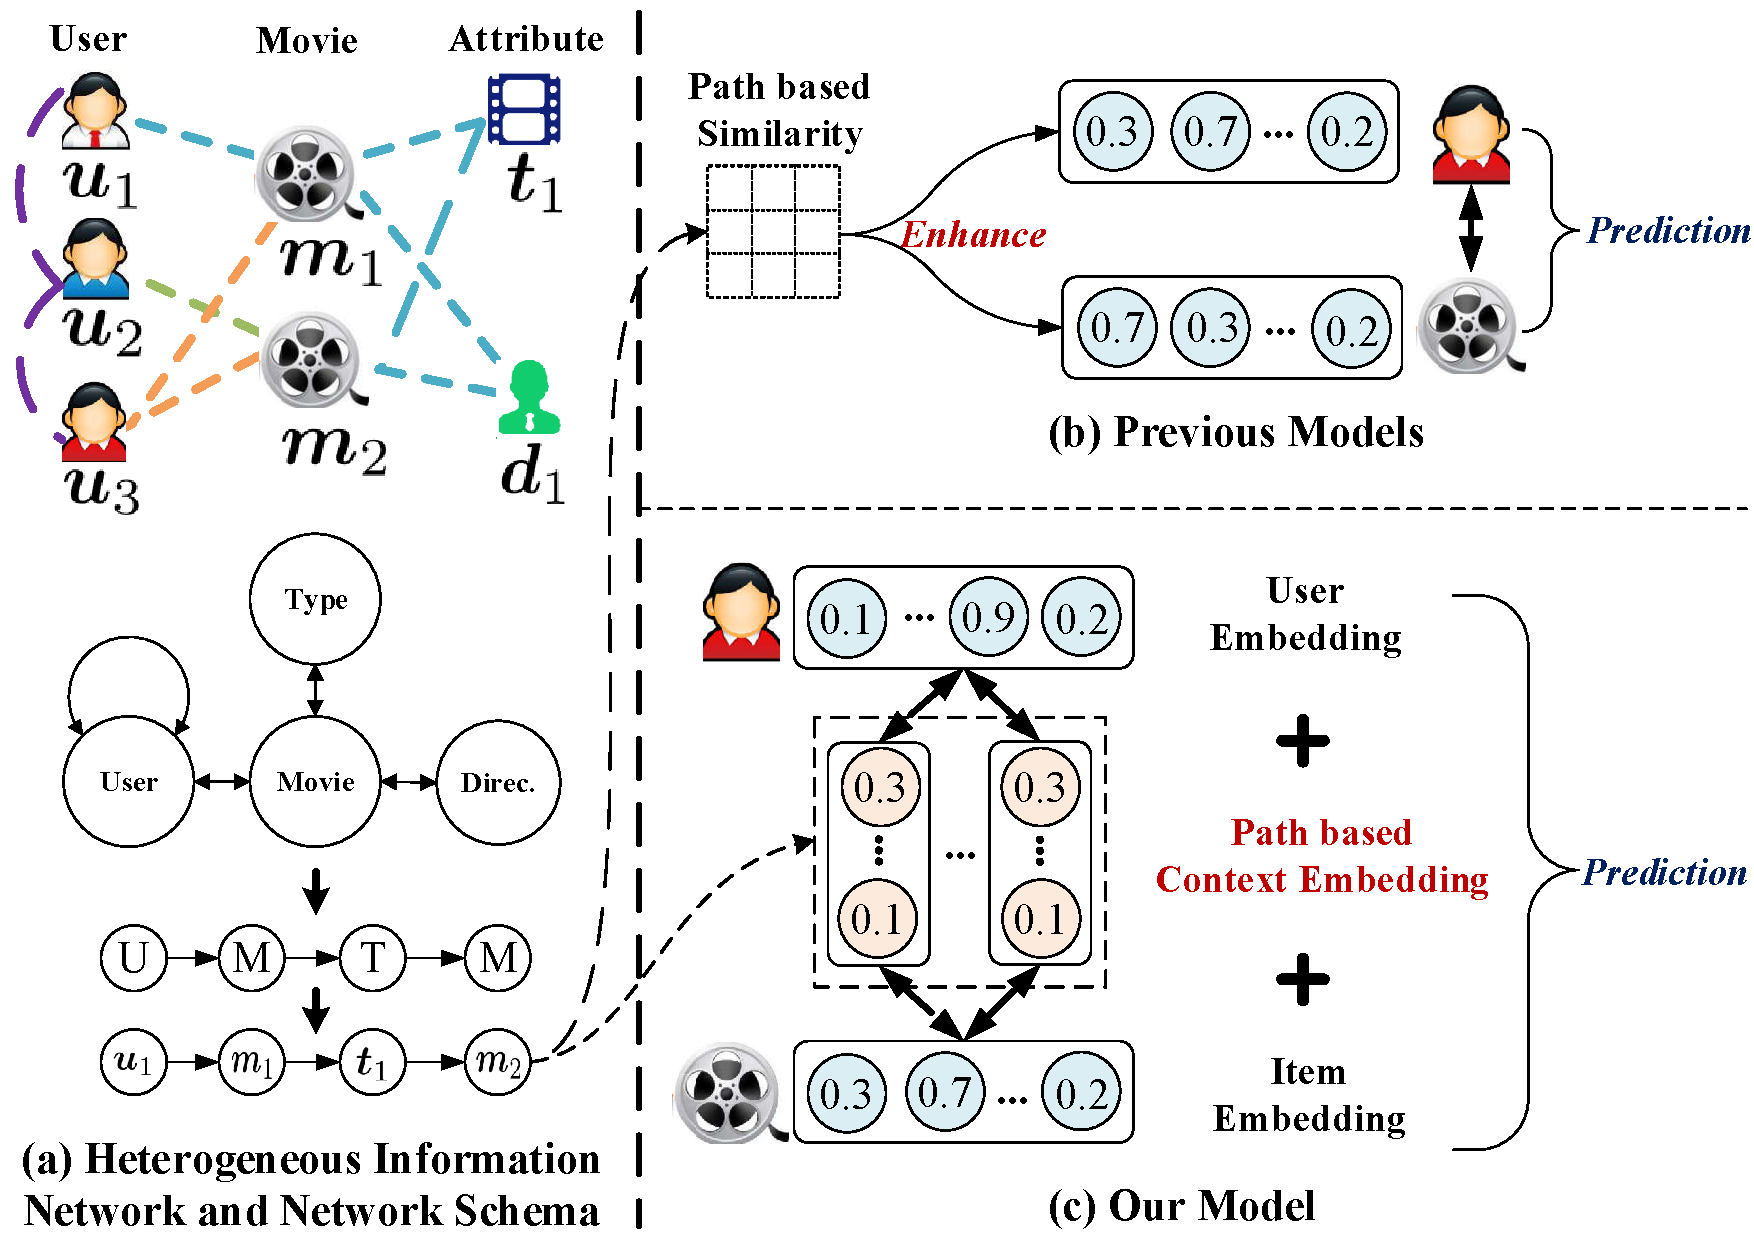
\includegraphics[width=8.5cm]{image/framework_intro.pdf}\\
  \caption{The illustration for HIN based recommendation setting (network schema, meta-path, path instance) and the comparison between our model and previous methods (two-way interaction \emph{v.s.} three-way meta-path based interaction). }\label{fig-framework-intro}
\end{figure}

To address these issues, we aim to leverage rich meta-path information from HIN for top-$N$ recommendation in a more principled way. For convenience,  given a target user-item pair, we call the aggregate meta-paths (together with their corresponding path instances) connecting the user with the item \emph{meta-path based context} of the interaction.
Our main idea is to (1) learn explicit representations for  meta-path based context tailored for the recommendation task, and (2) characterize a three-way interaction of the form:  $\langle$\emph{user}, \emph{meta-path}, \emph{item}$\rangle$. The paradigm of our work is illustrated in Fig.~\ref{fig-framework-intro}(c).
By explicitly incorporating meta-paths into the interaction model,  our approach is able to effectively mine and extract useful information from meta-path based context for improving the recommendation performance.
In this way, the characterization of  meta-path based context will be more flexible to adapt to different interaction scenarios, providing a good
interpretability on the recommendation results, \ie \emph{who} will adopt \emph{what} given the \emph{context}.
The idea is appealing, while the solution is challenging.  We have to consider three key research problems: (1) how to design the base architecture that is suitable for the complicated HIN based interaction scenarios; (2) how to generate meaningful path instances for constructing high-quality meta-path based context; and (3) how to capture the mutual effect between the involved user-item pair and meta-path based context in an interaction.

In this paper, for tackling various complicated interaction scenarios,  we adopt deep neural networks to build the base architecture for our recommender, since it has been shown that deep neural networks are more capable of learning arbitrary interaction function from data~\cite{he2017neural}.
We elaborately design a three-way neural interaction model by explicitly incorporating meta-path based context into the interaction.
 To construct the meta-path based context, we propose to use a 
 priority based sampling technique to select high-quality path instances for recommendation, since a simple meta-path guided sampling strategy like that in \cite{dong2017metapath2vec} is likely to generate low-quality path instances or even noise for our task.  Our model needs to learn the representations for users, items and meta-path based context.
We propose a novel co-attention mechanism to mutually improve the representations for  meta-path based context, users and items. Specially, the  representations for meta-path based context are first improved according to the information from a user-item pair in an interaction, and then user and item representations are further enhanced conditioned on the improved representations of meta-path based context.
 In this way,  the  meta-path based context are transformed into a form that is directly useful for a specific interaction, which is supposed to be more effective in recommendation than original representations.
Meanwhile, the improved user and item representations also embody useful evidence from calibrated meta-path based context for the current interaction.
By comparing Fig.~\ref{fig-framework-intro}(b) and (c),
we can see that, different from previous methods, our proposed model explicitly incorporates the meta-path based context into the interaction, and learns interaction-specific representations for these useful information.

%Our main idea is to learn interaction-specific representations for \emph{meta-path based context} in recommendation, and the learned  representations  are  involved as an explicit factor for modeling user-item interactions. We consider meta-paths as interaction context to bridge a user and an item, and characterize a three-way interaction of the form:  $\langle$ \emph{user}, \emph{meta-path}, \emph{item} $\rangle$.
%By explicitly learning interaction-specific meta-path representations,  the proposed approach is more adaptive and effective in modeling varying user-item interactions. In addition, by framing meta-path based information as interaction context, the approach is expected to have good model interpretability on the recommendation results, \ie \emph{who} will adopt \emph{what} given the \emph{context}.
%Since the recommendation task in HIN is usually complicated and difficult, we develop our approach based on the recent neural collaborative filtering framework~\cite{he2017neural} in implementing a powerful interaction function.
%Different from   \cite{he2017neural}, our interaction function is able to characterize three-way interaction by incorporating an explicit representation factor for the involved meta-path contexts in an interaction.
%The idea is intuitive, while the solution is challenging.  To implement the idea, we have to consider (1) how to generate useful interaction-specific path instances from some meta-path, and (2) how to make the meta-path representation adaptive to a specific  interaction.

%For the first problem, we find that using a simple meta-path guided sampling strategy like that in \cite{dong2017metapath2vec} is not effective to generate useful paths as interaction contexts.  The reason is that HIN is usually highly connected and contains many path instances for a single meta-path. Among these path instances, it is likely that only a few contain useful evidence for a single interaction.
%Based on this consideration, we pretrain a classic recommendation model with implicit feedback, \ie the Bayesian Personalized Ranking model (BPR)~\cite{rendle2009bpr},  for guiding the path generation process.  A path will be sampled only if it is consistent with the relevance evidence from the BPR model.

%borrow the \emph{pretrain} idea for training neural networks, and improve the sampling strategy by incorporating a heuristic method which are guided by both meta-paths and pretrained traditional implicit recommendation methods, \ie BPR~\cite{rendle2009bpr}.
%We force the sampling process to follow the path which is more consistent to the relevance evidence from BPR.

%For the second problem, we carefully design a hierarchical meta-path representation method. It first embeds a single path instance,  then represents a single  meta-path based on multiple  embeddings of its path instances, and finally aggregates multiple meta-path embeddings as the representation of the meta-path based context.  The most difficult point lies in how to make the representations of  meta-path based context flexibly adapt to varying interactions,  providing high-quality recommendation evidence. To solve this problem, we propose a novel co-attention mechanism to alternatively improve the representations for  meta-path based context, users and items. Specially, our  representations for meta-path based context are first improved according to the information from a user-item pair in an interaction, and then user and item representations are further enhanced according to the improved representations of meta-path based context. In this way,  the  meta-path based context are transformed into a form that is directly useful for a specific interaction, which is supposed to be more effective in recommendation than original representations. In addition, the improved user and item representations also embody useful evidence from elaborated meta-path based context.

To our knowledge, it is the first time that  meta-path based context has been explicitly modeled in a three-way neural interaction model, \ie $\langle$\emph{user}, \emph{meta-path}, \emph{item}$\rangle$, for the task of top-$N$ recommendation in HIN.
We propose a novel deep neural network with the co-attention mechanism by leveraging rich meta-path based context, which is able to learn interaction-specific representations for users, items and meta-path context.
We do extensive experiments on three real-world datasets, which demonstrate the effectiveness of the proposed model compared to the state of arts.
In addition, we also validate that the proposed model has the potential to alleviate cold-start problem and provide interpretable recommendation results.

%We construct extensive experiments on three real-world datasets demonstrate the effectiveness of the proposed model. Moreover, we show the capability of the proposed model for the cold-start prediction problem, and reveal that the impact of different meta-paths for recommendation via the proposed attention mechanism.


%For the above issues, it is challenging to develop a way to effectively extract and represent useful information for HINs due to data heterogeneity. Unlike previous studies using meta-path based similarities\cite{yu2013collaborative,zhao2017meta}, our idea is to learn effective representations between users and items for summarizing important structural characteristics and properties of HINs. Hence, we propose a new heterogeneous network embedding method to embed the relation between users and items. Considering heterogeneous characteristics and rich semantics reflected by meta-paths, we introduce a heuristic random walk guided by meta-paths to sample path instances (node sequences) between users and items. For each path instance, we learn a unique embedding representation representation for a user-item pair by convolution neural network. According to the assumption that the important feature in each embedding usually has high value, we utilize the max pooling layer to fuse the multiple embeddings \wrt different path instances as the output of CNN.

%After obtaining the user embeddings, item embeddings and the relation representation between users and items, we study how to integrate and utilize such information for top-$N$ recommendation. Traditional recommendation methods usually only consider the interaction between users and items, and utilize simple multiplication to uncover this complex interaction. Instead, we propose and explore the interaction between users, items and the user-item pairs and apply deep model (MLP) to model their interaction in order to endow the model a large level of flexibility and non-linearity for recommendation. For the interaction between users, items and user-item pairs, we proposed a novel neural attention mechanism for the fusion of path embedding under different meta-paths and the adjustments of user and item embeddings, respectively.
%
%By integrating the above description together, this work presents a novel meta-path based recommendation model. The proposed model first extract user-item pair's embedding according to meta-path in the HIN and encode users and items as well. And then we utilize neural attention mechanism to characterize the interaction of users and items for the top-$N$ recommendation. Extensive experiments on three real-world datasets demonstrate the effectiveness of the proposed model. We also verify the ability of the proposed mode to alleviate cold-start problem and examine the impact of meta-paths on performance. The key contributions of this paper can be summarized as follows:

%\textbullet\ We proposed a novel deep model for top-$N$ recommendation based on heterogeneous information networks to leverage rich information and semantics in RS. To our best knowledge, it is the first attempt to exploit structure information in HIN with the neural network for top-$N$ recommendation.

%\textbullet\ The proposed HeteRank model designs a deep neural network to learn the embedding of node pair, which is seldom studied in previous HIN embedding. Different from widely used path based random walk strategy in HIN embedding, we design a similarity guided  random walk strategy based on meta path, which can effectively capture structure features with less time cost.

%\textbullet\ We firstly propose a cooperative attention mechanism to fuse different embeddings for recommendations.  The cooperative attention mechanism utilizes the embedding of users and item for the better pair embedding, and leverages the pair embedding to make the embedding of users and items more suitable for recommendation.

%\textbullet\ Extensive experiments on three real-world datasets demonstrate the effectiveness of the proposed model. Moreover, we show the capability of the proposed model for the cold-start prediction problem, and reveal that the impact of different meta-paths for recommendation via the proposed attention mechanism.


\section{Related Work}
%In this section, we will review the related studies in three aspects, namely recommender systems, heterogeneous information networks and neural attention mechanism.
In the literature of recommender systems, early works mainly adopt collaborative filtering (CF) methods (\eg matrix factorization) to utilize historical interactions for recommendation~\cite{koren2009matrix}. Since CF methods usually suffer from cold-start problem, many works attempt to leverage additional information for recommendation, such as social information~\cite{wang2016social,zhao2014we,zhao2016connecting}, location information~\cite{yin2013lcars}, and heterogeneous information~\cite{feng2012incorporating}.
In addition, there are also some general feature based frameworks for incorporating context information for recommendation~\cite{rendle2010factorization,chen2012svdfeature,he2017neural2}.
 Recently, deep network models are also employed to extract refined latent features~\cite{he2017neural} from the user-item interaction data. 


As a newly emerging direction, heterogeneous information network~\cite{shi2017survey} can naturally model complex objects and their rich relations in recommender systems, in which objects are of different types and links among objects represent different relations~\cite{sun2011pathsim,shi2014hetesim}. 
Due to the flexibility of  HIN in modeling  various kinds of heterogenous data, it has been adopted
  in recommender systems to model rich auxiliary data.
Most of HIN based methods usually utilize path based similarity to enhance the representations of users and items, including meta-path based latent features~\cite{yu2014personalized}, meta-path based user similarity~\cite{shi2015semantic,liu2017personalized} and 
meta-graph based latent features~\cite{zhao2017meta}.  However, they seldom learn explicit representation for path or meta-path tailored to the recommendation task
%Yu et al.~\cite{yu2014personalized} introduce meta-path based latent features to represent the connectivity between users and items. Shi et al.~\cite{shi2015semantic} propose the concept of weighted heterogeneous information network and employ the meta-path based similarity of users for personalized recommendation. Recently, Zhao et al.~\cite{zhao2017meta} propose a factorization machine based model integrated with meta-graph based similarity for recommendation. 

On the other hand, network embedding has shown its potential in structure feature extraction and has been successfully applied in many data mining tasks. For example, Deepwalk~\cite{perozzi2014deepwalk} and node2vec~\cite{grover2016node2vec} combine random walk and skip-gram to learn network representations. Most of network embedding methods focus on homogeneous networks, and thus they cannot directly be applied to heterogeneous networks. Recently, attention is increasingly shifting towards heterogeneous networks.  Xu et al.~\cite{xu2017embedding} propose an Embedding of Embedding model to encode the intra-network and inter-network edges for the coupled heterogeneous network. Dong et al.~\cite{dong2017metapath2vec} obtain the neighbors of a node via meta-paths and learn the HIN embedding by skip-gram with negative sampling. Furthermore, Fu et. al~\cite{Fu2017HIN2Vec} learn node embedding to capture rich relation semantics in HIN via neural network model. Although these HIN embedding methods has shown their effectiveness in some tasks, they usually focus on general node embeddings, seldom considering the path embedding for the recommendation task.

%As a newly emerging direction, heterogeneous information network~\cite{shi2017survey} can naturally model complex objects and their rich relations in recommender systems, in which objects are of different types and links among objects represent different relations~\cite{sun2013mining}. And several path-based similarity measures~\cite{sun2011pathsim,shi2014hetesim} are proposed to evaluate the similarity of objects in heterogeneous information network. Therefore, some researchers have began to be aware of the importance of HIN-based recommendation. Wang et al.~\cite{feng2012incorporating} propose the OptRank method to alleviate the cold-start problem by utilizing heterogeneous information contained in social tagging system. Furthermore, the concept of meta-path is introduced into hybrid recommender systems~\cite{yu2013recommendation}. Yu et al.~\cite{yu2013collaborative} utilize meta-path-based similarities as regularization terms in the matrix factorization framework. Yu et al.~\cite{yu2014personalized} take advantage of different types of entity relationships in heterogeneous information network and propose a personalized recommendation framework for implicit feedback dataset. Luo et al.~\cite{luo2014hete} propose a collaborative filtering based social recommendation method using heterogeneous relations. More recently, Shi et al.~\cite{shi2015semantic} propose the concept of weighted heterogeneous information network and design a meta-path based collaborative filtering model to flexibly integrate heterogeneous information for personalized recommendation. In \cite{shi2016integrating}, the similarities of users and items are both evaluated by path based similarity measures under different semantic meta-paths and a matrix factorization based on dual regularization framework is proposed for rating prediction. Most of HIN-based methods rely on the path based similarity, which may not fully mine latent features of users and items on HINs for recommendation.

Our work is inspired by the recent progress of neural attention mechanism in the fields of computer vision~\cite{xu2015show} and natural language processing~\cite{phan2017neupl}. In particular, co-attention or cross-attention mechanisms have been applied to solve complicated NLP tasks~\cite{hao2017end,xiong2016dynamic}.
We are also aware of the application of attention mechanism in recommender systems~\cite{chen2017attentive,wang2017dynamic,xiao2017attentional}.
We borrow the idea of co-attention mechanisms for modeling mutual effect between the meta-path and the involved user-item pair in an interaction.
To our knowledge, it is the first time that meta-path based context has been explicitly modeled in a three-way neural interaction model with the co-attention mechanism.
%, which has a totally different task goal.

% Its success is mainly due to the reasonable assumption that human recognition does not tend to process a whole signal in its entirety at once; instead, one only focuses on selective parts of the whole perception space when and where as needed.

%Recently, some co-attention mechanisms have been proposed to solve more complex interaction in NLP. For example, Hao et al.~\cite{hao2017end} propose a novel cross-attention to improve the representation of the question and answer for KB-QA. Xiong et al.~\cite{xiong2016dynamic} present a co-attention mechanism that attends to the question and document simultaneously and fuse both attention contexts for QA task. Inspired by these methods, our MCRec designs a hierarchical co-attention structure for recommendation tasks.



\section{Preliminaries}
%In this section, we will first clarify the background and some preliminary knowledge of this study, and then present our recommendation problem in detail.

%\subsection{User Implicit Feedback}
In this paper, we consider the recommendation task targeting for implicit feedback. With $n$ users $\mathcal{U} = \{u_1, ..., u_n\}$ and $m$ items $\mathcal{I} = \{i_1, ..., i_m\}$, we define each entry $r_{u,i}$ in the user implicit feedback matrix $\mathbf{R} \in \mathbb{R}^{n \times m}$ as follows: $r_{u,i}=1$ when $\langle u, i \rangle$ interaction is observed, and $r_{u,i}=0$ otherwise.
Here the value of 1 in the matrix $\mathbf{R}$ indicates the interaction result between a user and an item, \eg whether a user has watched or rated a movie. %However, the value of 1 in the implicit feedback data does not mean users actually like the items. Actually a user watched a movie because he is interested in the movie but he might probably dislike the movie and give a low rate to the movie. Similarly, the value of 0 does not necessarily mean the users dislike the items, it also can be regarded as potential interactions (users are not aware of the items).

%\subsection{Heterogeneous Information Network}
We frame our recommendation task in the setting of heterogeneous information network, which can be defined as follows:

%A heterogeneous information network (HIN) is a special kind of information network containing multiple types of objects or multiple types of links,
\begin{myDef}
\textbf{Heterogeneous Information Network}~\cite{sun2011pathsim}. A HIN is defined as a directed graph ${\mathcal{G}} = (\mathcal{V}, \mathcal{E})$ with an entity type mapping function $\phi : \mathcal{V} \rightarrow \mathcal{A}$ and a link type mapping function $\varphi : \mathcal{E} \rightarrow \mathcal{R}$. $\mathcal{A}$ and $\mathcal{R}$ denote the sets of predefined entity and link types, where $|\mathcal{A}| + |\mathcal{R}| > 2$.
\end{myDef}

In HIN,  \textbf{network schema} is proposed to describe the meta structure of a network, which illustrates the object types and their interaction relations.
\begin{exmp}
Fig.~\ref{fig-framework-intro}(a) illustrates a HIN example and its corresponding network schema for movie recommender system. We can see that the network consists of multiple types of
objects (\eg User ($U$), Movie ($M$), Director ($D$)) and their semantic relations (\eg watching relation between users and movies, friend relation among users, and directed by relation between movies and directors).
\end{exmp}

In HIN, two objects can be connected via different semantic paths, which are defined as meta-paths.
\begin{myDef}
\textbf{Meta-path}~\cite{sun2011pathsim}. A meta-path $\rho$ is defined as a path in the form of $\mathcal{A}_1 \xrightarrow{\mathcal{R}_1} \mathcal{A}_2 \xrightarrow{\mathcal{R}_2} \cdots \xrightarrow{\mathcal{R}_l} \mathcal{A}_{l+1}$ (abbreviated as $\mathcal{A}_1\mathcal{A}_2 \cdots \mathcal{A}_{l+1}$), which describes a composite relation $\mathcal{R}_1 \circ \mathcal{R}_2 \circ \cdots \circ \mathcal{R}_l$ between object $\mathcal{A}_1$ and $\mathcal{A}_{l+1}$, where $``\circ"$ denotes the composition operator on relations.
\end{myDef}

Giving a meta-path $\rho$, there exist multiple specific paths under the meta-path, which is called a \textbf{path instance} denoted by $p$.  As we have illustrated above, the implicit feedback matrix $\mathbf{R}$ indicates the interaction result between a user  and an item. We are particularly interested in the meta-paths that connect a user and an item in HIN, which can reveal semantic context for a user-item interaction.

%, while a pair of $\langle user, item \rangle$ can be indirectly connected via different meta-paths, which reflects different types of interactions between users and items. The aggregated meta-paths constitute the context of a $\langle user, item \rangle$ pair, which can comprehensively reveal the semantic relations of the user and item.
\begin{myDef}
\textbf{Meta-path based Context}. Giving a user $u$ and an item $i$, the meta-path based context  is defined as the aggregate set of path instances under the considered meta-paths connecting the two nodes on the HIN.
\end{myDef}

\begin{exmp}
Take Fig.~\ref{fig-framework-intro}(a) as an example. The user $u_1$ and movie $m_2$ can be connected via multiple meta-paths, $\eg$ ``$u_1$-$m_1$-$u_3$-$m_2$" ($UMUM$) and  ``$u_1$-$m_1$-$t_1$-$m_2$" ($UMTM$), which constitute the context of the interaction $\langle u_1, m_2 \rangle$. Different meta-paths usually convey different interaction semantics of $\langle u_1, m_2 \rangle$. For example, $UMUM$ and $UMTM$  paths indicate that user $u_1$ has watched  movie $m_2$ since (1) a user $u_2$ sharing the same watching records (\ie $m_1$) has watched $m_2$ and (2) she/he has previously watched movie $m_1$ with the same type of movie $m_2$ respectively.
These meta-path based contexts reveal varying interaction semantics through aggregating different meth-paths.
\end{exmp}

%\subsection{Problem Definition}
%Recently, HIN has widely been used to model various complex interaction systems~\cite{shi2017survey}. Specially, it has been adopted in recommender systems for characterizing complex and heterogenous recommendation settings.
Given the above preliminaries, we are ready to define our task.

\begin{myDef}
\textbf{HIN based Top-$N$ Recommendation}. Given a heterogeneous information network $\mathcal{G}$ with user implicit feedback matrix $\mathbf{R}$, for each user $u \in \mathcal{U}$, we aim to recommend a ranked list of items that are of interest to $u$.
\end{myDef}

Many efforts have been made for HIN based recommendation. While, most of these works focus on the rating prediction task, which predicts the absolute preference score of a user to a new item~\cite{zhao2017meta,shi2015semantic}. Top-$N$ recommendation task is more common in practice, since implicit feedback is easier to obtain.

\section{The Proposed Model}

In this section, we present the proposed  model that leverages  Meta-path based Context for RECommendation, called \textbf{MCRec}.
%Our MCRec model characterizes the interaction between users and items with the incorporation of meta-paths as context.


%extends the neural collaborative filtering framework~\cite{he2017neural} by incorporating meta-path based context. The meta-path based context is first modeled by a hierarchical embedding method, and then improved with the co-attention mechanism.


\subsection{Model Overview}
Different from existing HIN based recommendation models, which only learn the representations for users and items,  we explicitly incorporate meta-paths as the context  in an interaction between a user and an item.
Instead of modeling the two-way interaction $\langle user, item \rangle$, we aim to characterize a three-way interaction
$\langle \emph{user}$, \emph{\text{meta-paths}}, $\emph{item} \rangle$.
For learning a better interaction function that generates the recommendations, we learn the representations (\ie embedding) for users, items and their interaction contexts, which is the aggregated meta-paths.
We present the overall architecture for the proposed model in Fig.~\ref{fig-framework-model}.
As we can see, besides the components for learning user and item embeddings, the most important part lies in the embedding of \emph{meta-path based context}. The meta-path based context is first modeled into a low-dimensional embedding using a hierarchical neural network.
With the initially learned embeddings for users, items and meta-path based context, the co-attention mechanism further improves the three representations through alternative enhancement. Due to the incorporation of  meta-path based context, our model is expected to yield a better performance and also improve the interpretability for recommendation results.

\begin{figure}
  \centering
  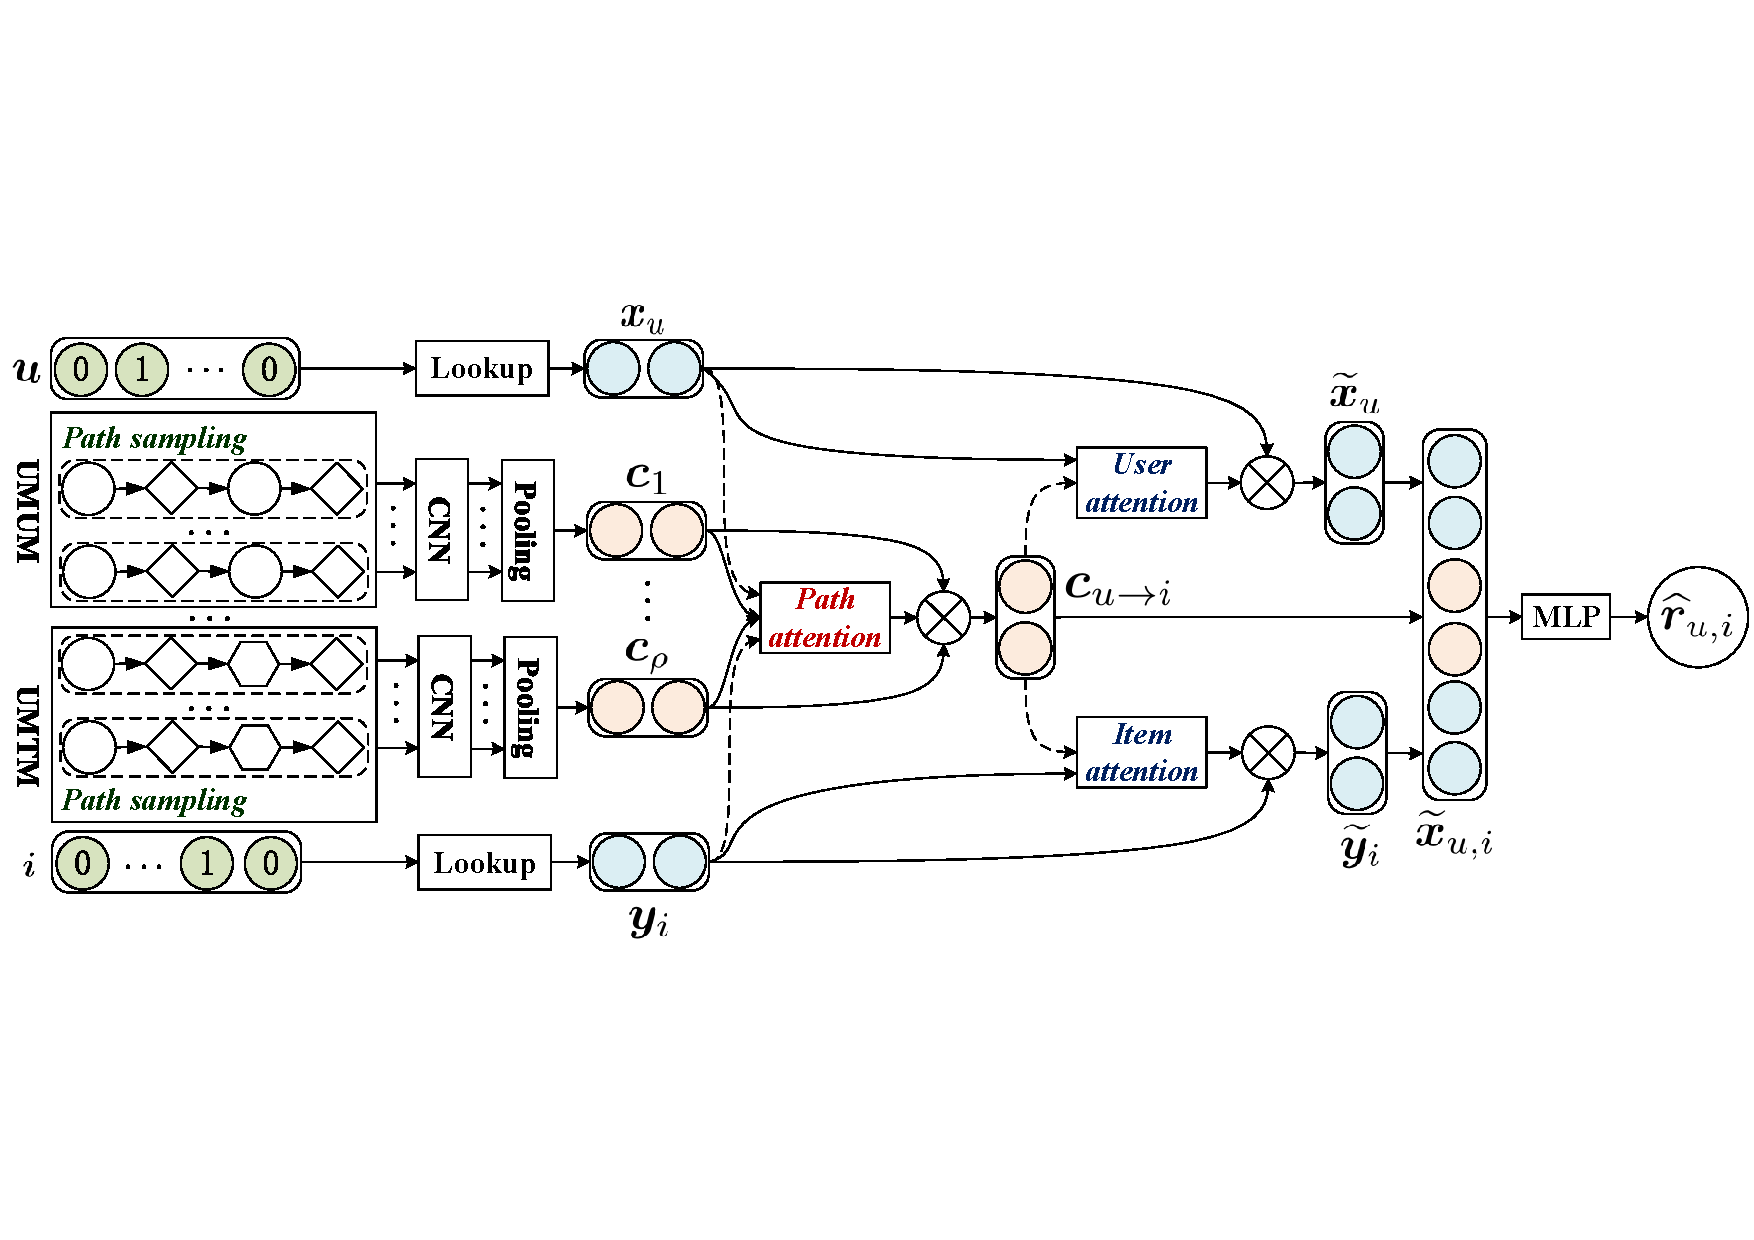
\includegraphics[width=8.5cm]{image/framework_model.pdf}\\
  \caption{The overall architecture of the proposed model.}\label{fig-framework-model}
\end{figure}

%we  propose a \emph{M}eta-path based \emph{C}context embedding model for top-N \emph{Rec}ommendation (called MCRec). The basic idea of MCRec is that, except the embedding of users and items, MCRec learns the context embedding of a $\langle user, item \rangle$ pair through fusing the meta-path embeddings connecting the user and item, and then exploits the correlations of the embeddings of users, items,  and their context. As illustrated in Fig.~\ref{fig-framework-model}, MCRec includes two main components: learn embeddings of users, items, and their context, and fuse embeddings. In the context embedding phrase, MCRec first learns path embedding for each meta-path connecting a user $u$ and item $i$, and then fuse these multiple path embeddings for the context of the $\langle u, i\rangle$ with the help of the embeddings of user $u$ and item $i$. In the embeddings fusing phrase,  the embeddings of user $u$, item $i$, and  $\langle u, i\rangle$ context enhance each other with a co-attention network. In the following sections, we will present the details of these components.

\subsection{User and Item Embedding}

Following~\cite{he2017neural}, we set up a lookup layer to transform the one-hot representations of users and items into
 low-dimensional dense vectors, called \emph{embeddings}. Formally, given a user-item pair $\langle u, i \rangle$, let
 $\mathbf{p}_u \in \mathbb{R}^{|\mathcal{U}| \times 1}$ and $\mathbf{q}_i \in \mathbb{R}^{|\mathcal{I}| \times 1}$ denote their one-hot representations.  The lookup layers correspond to two parameter matrices $\mathbf{P} \in \mathbb{R}^{|\mathcal{U}| \times d}$ and $\mathbf{Q} \in \mathbb{R}^{|\mathcal{I}| \times d  }$, which store the latent factors for users and items respectively.  Here $d$ is the dimension size of user and item embeddings, and $|\mathcal{U}|$ and $|\mathcal{I}|$ are the total number of users and items respectively.
 The lookup operation is implemented as follows:
 \begin{eqnarray}
\mathbf{x}_u &=& \mathbf{P}^{\top} \cdot \mathbf{p}_u, \label{equ-userembedding}\\
\mathbf{y}_i &=& \mathbf{Q}^{\top} \cdot \mathbf{q}_i. \label{equ-itemembedding}
\end{eqnarray}

%Similar to previous HIN based recommendation models, the MCRec first learns the embedding of users and items, as shown in two sides of Fig. \ref{fig-framework-model}. The proposed model accepts a user-item pair $\langle u, i \rangle$ as input. We represent the involved user $u$ and item $i$ as one-hot vectors corresponding to a unique index key belonging to user $u$ and item $i$, $\eg$ $\mathbf{p}_u \in \mathbb{R}^{|\mathcal{U}| \times 1}$ and $\mathbf{q}_i \in \mathbb{R}^{|\mathcal{I}| \times 1}$. In the embedding layer, these one-hot vectors can be transformed to low-dimensional real-value representations. In order to embed users and items, we introduce two parameter matrices $\mathbf{P} \in \mathbb{R}^{d \times |\mathcal{U}|}$ and $\mathbf{Q} \in \mathbb{R}^{d \times |\mathcal{I}|}$ which store the latent factors for users and items respectively. Here $d$ is the dimension of user and item embeddings, while $|\mathcal{U}|$ and $|\mathcal{I}|$ are the total number of users and items respectively. By applying a lookup layer, we can obtain the embeddings of users and items as follows:


\subsection{Characterizing Meta-path based Context for Interaction}
A major novelty of our work is to explicitly characterize meta-path based context for improving the modeling of the  interaction.
In this part, we first study how to generate high-quality path instances, and then present how to learn effective representations (\ie embeddings) for meta-path based context.

%Different from HIN based recommendation models and HIN embedding methods, we designs a novel meta-path based context embedding to exploit the rich semantic interactions between users and items through fusing multiple path embeddings, as shown in the middle of  Fig. \ref{fig-framework-model}. The MCRec first samples several path instances based on a given meta-path with a novel heuristic random walk strategy, and then embeds these path instances with a CNN layer. After that, the embedding of this meta-path can be obtained through fusing these path instance embeddings. Finally, we give a naive context embedding strategy to fuse multiple meta-path embeddings.

\subsubsection{Sampling Path Instances via Priority based Random Walk based on Meta-paths}
Existing HIN embedding models mainly adopt a meta-path guided random walk strategy to generate path instances~\cite{dong2017metapath2vec}, relying on a uniform sampling over the out-going nodes.
However, the path instances generated by such a simple random walk strategy are usually of low quality and even accompanied with much noise, which makes the sampling strategy unsuitable for recommendation.
Intuitively, at each step, the walker should  wander to a neighbor of a higher ``priority'' score with a larger probability, since such an out-going node can reflect more reliable semantics by forming a more close link. Hence, the key problem is how to define the priority score of an out-going node.
Inspired by the tricks for training neural networks~\cite{he2017neural,hinton2012better}, we propose to use a similar \emph{pretrain} technique to measure the priority degree of each candidate out-going nodes.  The basic idea is to first learn a latent vector for each node with historical user-item interaction records by using traditional matrix factorization method without meta-path information. Then, we can measure the priority degree by the similarity between the current node and candidate out-going nodes.  Such a priority score directly reflects the association degree between two nodes. To pretrain the latent factors for all the entities in HIN, we train the feature based matrix factorization framework SVDFeature~\cite{chen2012svdfeature}, adapted to implicit feedback with the pairwise loss in~\cite{rendle2009bpr}, on all the available historical interaction records.  SVDFeature is able to characterize various kinds of context information. We can incorporate the entities from HIN related to an interaction as the context of a training instance. With the learned latent factors, we can compute the pairwise similarities between two consecutive nodes along a path instance, and then average these similarities for ranking the candidate path instances. Finally, given a meta-path, we only keep top $K$ path instances with the highest average similarities.

%In our recommendation task, users and items are the two core entity types, and the key part is the out-going link of the forms $user \rightarrow item$ and $item \rightarrow user$.
%We adopt the widely used Bayesian Personalized Ranking model (BPR) with implicit feedback to learn both user and  item latent factors.
%Given a user node and item node, we use the inner product between their corresponding latent factors as the link importance.
%For each walk with the forms $user \rightarrow item$ and $item \rightarrow user$, we sample the candidate node according to their link importance
%with the current node.  Note that we don't consider compute the importance for links with  other forms, \eg $item  \rightarrow type $ or $user  \rightarrow type$, since we have found that the links between user and item nodes play the key role in generating high-quality path instances.
%While, our approach can be easily extended to compute a full-path importance score by learning a latent factor for each kind of entities, \eg using Factorization Machine~\cite{rendle2010factorization}.  Given a meta-path, for efficiency consideration, we only keep top $K$ path instances with the highest average link importance.

%In order to learn the embedding of a user-item pair, we need to sample some path instances connect the user and item. In recent HIN embedding models \cite{}, meta-path based random walk strategy is widely employed to extract path instances, since meta-path can effectively extract features and embody rich semantics \cite{}. However?the path instances generated by a simple meta-path based random walk strategy usually be low-quality, accompanied with much noise, which makes this strategy not suitable for recommendation. We know that, in RS, there are a huge number of user-item pairs, so we can only sample a small number of path instances for each user-item pair. For the specific requirement of RS, we propose a novel preference-guided random walk strategy based on meta-path to sample a small number of high-quality path instances that can effectively represent structure information of nodes. The basic idea is that we can let walkers wander to neighbors with the higher preference degree, since each node has  more close relation with its preferring neighbors. The preference degree can be simulated by the product of the latent factors of two nodes, where the latent factors can be calculated by factorizing the relation matrix of the adjacent two node types. Concretely, a walker wanders along the given meta-path, and selects the top-$l$ candidate neighbors with high preference degree in each step. After that, we select the top-$K$ path instances with high average of preference degree as samples. Although it is time-consuming for calculating the preference degree, the process can be done offline. In addition, we do not need to calculate the preference degree in each step. We just need to do preference selection on the ``user-item'' relation, since this relation is more important for recommendation. Experiments also validate that MCRec can achieve good performance with only 5 sampled path instances for each user-item pair.

\subsubsection{Meta-path based Context Embedding} After obtaining path instances from multiple meta-paths, we continue to study how to model these
meta-path based context as an informative embedding. Our method naturally follows a hierarchical structure: embedding a single path instance $\rightarrow$  embedding a single meta-path $\rightarrow$  embedding the aggregate meta-paths.

\paratitle{Path Instance Embedding}.  A path instance is essentially a sequence of entity nodes.
To embed such a node sequence into a low-dimensional vector, many methods can apply. Here, we adopt the commonly used Convolution Neural Network (CNN) to deal with sequences of variable lengths. Formally, given a path $p$ from some meta-path $\rho$, let $\mathbf{X}^{p} \in \mathbb{R}^{L \times d}$ denote the embedding matrix formed by concatenating node embeddings, where  $L$ is the length of the path instance and $d$ is the embedding dimension for entities. The structure of CNN consists of a convolution layer (producing new features with the convolution operation) and a max pooling layer. We learn the embedding of a path instance $p$ using CNN as follows:

\begin{equation} \label{equ-pathembedding}
\mathbf{h}_p = CNN(\mathbf{X}^{p}; \mathbf{\Theta})
\end{equation}
where $\mathbf{X}^{p}$ denotes the matrix of the path instance $p$ and $\mathbf{\Theta}$ denotes all the related parameters in CNNs.
%where $*$ denotes the convolution operator, $b_j$ is a bias term and $f$ is an activation function. In our work, we use Rectified Linear Units (ReLU) \cite{nair2010rectified}, which yields better than tanh unit and sigmoid unit in our empirical results. The ReLU unit is defined as follows.
%\begin{equation}\label{equ-relu}
%f(x) = max\{0, x\}.
%\end{equation}

\paratitle{Meta-path Embedding}. Since a meta-path can produce multiple path instances,  we further apply the max pooling operation to derive the embedding for a meta-path. Let $\{\mathbf{h}_p\}_{p = 1}^{K}$ denote the embeddings for the $K$ selected path instances from meta-path $\rho$.
The embedding $\mathbf{c}_\rho$ for meta-path $\rho$ can be given

\begin{equation} \label{equ-pooling}
\mathbf{c}_\rho = \text{max-pooling}(\{\mathbf{h}_p\}_{p = 1}^{K}).
\end{equation}
Our max pooling operation is carried out over $K$ path instance embeddings, which aim to capture the important dimension features from multiple path instances.

\paratitle{Simple Average Embedding for Meta-path based Context}. Finally, we apply the average pooling operation to derive the embedding for modeling the aggregate meta-path based context

\begin{equation} \label{equ-avg}
\mathbf{c}_{u \rightarrow i} = \frac{1}{|\mathcal{M}_{u \rightarrow i}|}\sum_{\rho \in \mathcal{M}_{u \rightarrow i} }\mathbf{c}_{\rho},
\end{equation}
where $\mathbf{c}_{u \rightarrow i}$ is the embedding for meta-path based context and $\mathcal{M}_{u \rightarrow i}$ is the set of the considered meta-paths for the current interaction. In this naive embedding method, each meta-path indeed receives equal attention, and
the representation of meta-path based context fully depends on the generated path instances.
It does not incorporate the involved user and item into consideration, which lacks the ability of capturing varying semantics from meta-paths in different interaction scenarios.

\subsection{Improving Embeddings for Interaction via Co-Attention Mechanism}
%Above, the embedding learning of meta-path based context does not take the involved user-item pair into consideration, which can't effectively capture the varying semantics of a  meta-path in different interaction scenarios.
%The above embedding method
Intuitively, different users are likely to have different preferences over the meta-paths.
Even for the same user, a meta-path may have varying semantics in her multiple interactions with different items.
A good embedding method for modeling meta-path based context should be interaction-specific,
which is able to provide highly discriminative semantics in various complicated recommendation scenarios.
Furthermore, in a user-item interaction, meta-paths provide important context information, and hence the involved user and item are likely to be affected
by such interaction context, too.
Based on these discussions, if we could improve the embeddings of users, items and meta-paths in a mutual enhancement way,
it may be possible to  develop a more effective representation learning method.
Inspired by the recent progress of attention mechanism made in computer vision and natural language processing~\cite{xu2015show,phan2017neupl},
we propose a novel co-attention mechanism to achieve this goal.


%could fully model the dependence between a user, an item and meta-paths in an interaction,  we may be able to develop an more effective representation learning method. Inspired by the recent progress of attention mechanism made in computer vision and natural language processing~\cite{mnih2014recurrent,phan2017neupl}, we propose a novel co-attention mechanism to achieve our goal.
%we should jointly learn the embeddings for meta-path, users, and items.
%the meta-path based context should be modeled accordingly in different interactions
%In this way, the embedding for modeling meta-path based context


\subsubsection{Attention for Meta-path based Context}
Since different meta-paths may have different semantics in an interaction, we learn the interaction-specific attention weights over meta-paths conditioned on the involved user and item.  Given the user embedding $\mathbf{x}_u$, item embedding $\mathbf{y}_i$, the  context embedding $\mathbf{c}_\rho$ for  a meta-path $\rho$, we adopt a two-layer architecture to implement the attention

\begin{eqnarray}
\bm{\alpha}^{(1)}_{u, i, \rho} &=& f(\mathbf{W}^{(1)}_u\mathbf{x}_u + \mathbf{W}^{(1)}_i\mathbf{y}_i + \mathbf{W}^{(1)}_{\rho}\mathbf{c}_{\rho} + \mathbf{b}^{(1)}), \label{equ-attention1}\\
\alpha^{(2)}_{u, i, \rho} &=& f({\mathbf{w}^{(2)}}^{\top} \bm{\alpha}^{(1)}_{u, i, \rho} + b^{(2)}), \label{equ-attention2}
\end{eqnarray}
where $\mathbf{W}^{(1)}_*$ and $\mathbf{b}^{(1)}$ denote the weight matrix and the bias vector for the first layer, and the $\mathbf{w}^{(2)}$ and $b^{(2)}$ denote the weight vector and the bias for the second layer. $f(\cdot)$ is set to the ReLU function.

The final meta-path weights are obtained by normalizing the above attentive scores over all the meta-paths using the softmax function, 

\begin{equation} \label{equ-attentinscore}
\alpha_{u, i, \rho} = \frac{\exp(\alpha^{(2)}_{u, i, \rho})}{\sum_{\rho' \in \mathcal{M}_{u \rightarrow i}}\exp(\alpha^{(2)}_{u, i, \rho'})}.
\end{equation}
which can be interpreted as the contribution of the meta-path $\rho$ to the interaction between $u$ and $i$.
After we obtain the meta-path attention scores $\alpha_{u, i, \rho}$, the new embedding for aggregate meta-path context can be given  as the following weighted sum:
\begin{equation}\label{equ-path}
\mathbf{c}_{u \rightarrow i} = \sum_{\rho \in \mathcal{M}_{u \rightarrow i}}\alpha_{u, i, \rho} \cdot \mathbf{c}_{\rho},
\end{equation}
where $ \mathbf{c}_{\rho}$ the learned embedding for the meta-path $\rho$ in Eq.~\ref{equ-pooling}.
Since the attention weights $\{ \alpha_{u, i, \rho} \}$ are generated for each interaction, they are interaction-specific and able to capture varying interaction context.

\subsubsection{Attention for Users and Items}
Given a user and an item, the meta-path connecting them provide important interaction context, which is likely to affect the original  representations
of users and items.  Giving  original user and item latent embeddings $\mathbf{x}_u$ and $\mathbf{y}_i$,
and the meta-path based context  embedding $\mathbf{c}_{u \rightarrow i}$ for the interaction between $u$ and $i$,
we use a single-layer network to compute the attention vectors $\bm{\beta}_u$ and $\bm{\beta}_i$  for user $u$ and item $i$ as,

\begin{eqnarray}
\bm{\beta}_u &=& f(\mathbf{W}_{u} \mathbf{x}_u + \mathbf{W}_{u \rightarrow i} \mathbf{c}_{u \rightarrow i} + \mathbf{b}_{u}), \label{equ-userattention}\\
\bm{\beta}_i &=& f(\mathbf{W}'_{i} \mathbf{y}_i + \mathbf{W}'_{u \rightarrow i} \mathbf{c}_{u \rightarrow i}+ \mathbf{b}'_{i}) \label{equ-itemattention},
\end{eqnarray}
where $\mathbf{W}_*$ and $\mathbf{b}_u$ denote the weight matrix and bias vector for user attention layer, $\mathbf{W}'_*$ and $\mathbf{b}'_i$ denote the weight matrix and bias vector for item attention layer. Similarly, $f(\cdot)$ is set to the ReLU function. Then, the final representations of user and item are computed by using an element-wise product ``$\odot$" with the attention vectors
\begin{eqnarray}
\tilde{\mathbf{x}}_u &=& \bm{\beta}_u \odot \mathbf{x}_u, \label{equ-user}\\
\tilde{\mathbf{y}}_i &=& \bm{\beta}_i \odot \mathbf{y}_i. \label{equ-item}
\end{eqnarray}
The attention vectors $\bm{\beta}_u$ and $\bm{\beta}_i$ are used for improving the original user and item embeddings conditioned on the calibrated meta-path based context $\mathbf{c}_{u \rightarrow i}$ (Eq.~\ref{equ-path}).

By combining the two parts of attention components, our model improves the original representations for users, items and meta-path based context in a mutual enhancement way.  We call such an attention mechanism \emph{Co-Attention}.
To our knowledge, few HIN based recommendation methods are able to learn explicit representations for meta-paths, especially in an interaction-specific way.


\subsection{The Complete Model}
Until now, given an interaction between user $u$ and item $i$, we have the embeddings for user $u$, item $i$ and the meta-path connecting them.
We combine the three embedding vectors into a unified representation of the current interaction as below:

\begin{equation}\label{equ-model}
\widetilde{\mathbf{x}}_{u,i} = \tilde{\mathbf{x}}_u \oplus \mathbf{c}_{u \rightarrow i} \oplus \tilde{\mathbf{y}}_i,
\end{equation}
where ``$\oplus$" denotes the vector concatenation operation, $\mathbf{c}_{u \rightarrow i}$  (Eq.~\ref{equ-path}) denotes the embedding  of the meta-path based context for $\langle u, i \rangle$, $\tilde{\mathbf{x}}_u$ (Eq.~\ref{equ-user}) and $\tilde{\mathbf{y}}_i$ (Eq.~\ref{equ-item}) denote the improved embeddings of user $u$ and item $i$ respectively.
$\widetilde{\mathbf{x}}_{u,i}$ encodes the information of an interaction from three aspects: the involved user, the involved item and the corresponding meta-path based context.
Following~\cite{he2017neural}, we feed $\widetilde{\mathbf{x}}_{u,i}$ into a MLP component in order to implement a nonlinear  function for modeling complicated interactions

\begin{equation} \label{equ-predict}
\hat{r}_{u,i} = \text{MLP}(\widetilde{\mathbf{x}}_{u,i}),
\end{equation}
where the MLP component is implemented with two hidden layers with ReLU as the activation function and an output layer with the sigmoid function.
With the premise that neural network models can learn more abstractive features of data via using a small number of hidden units for higher layers~\cite{he2016deep}, we empirically implement a tower structure for the MLP component, halving the layer size for each successive higher layer.

Defining a proper objective function for model optimization is a key step for learning a good recommendation model. Traditional point-wise recommendation models  for the rating prediction task usually adopt the squared error loss~\cite{koren2009matrix}. While, in our task, we have only implicit feedback available.  Following \cite{he2017neural,tang2015line}, we learn the parameters of our model with negative sampling and the objective for an interaction $\langle u, i \rangle$ can be formulated as follows:

\begin{equation} \label{equ-loss}
\ell_{u, i} = - \log \hat{r}_{u,i} - {E_{j \sim P_{neg}}[\log(1 - \hat{r}_{u,j})]},
\end{equation}
where the first term models the observed interaction, and the second term models the negative feedback drawn from the noise distribution $P_{neg}$.
 In this paper, we set the distribution $P_{neg}$ as uniform distribution, which is flexible to extend to other biased distributions, \eg popularity based distribution.
 
As shown in Eq. \ref{equ-model},  MCRec is a flexible approach to leveraging heterogeneous information. If we remove the term $\mathbf{c}_{u \rightarrow i}$ from Eq. \ref{equ-model}, MCRec degrades into the neural collaborative filtering model without HIN based information, \ie NeuMF~\cite{he2017neural}. Our approach is general to work with any methods that are able to learn $\mathbf{c}_{u \rightarrow i}$.
For a recommendation method, we are more concerned about the online prediction time than the offline training time. 
Compared with NeuMF, the additional online-recommendation time cost  from our approach mainly lies in the step of generating path instances, since it is relatively cheap to compute path embeddings using CNN and max pooling operations which is easy to be accelerated in parallel.  
For efficiency consideration, we use a small number $l$ of meta-paths. 
With the network schema, we can offline obtain all the possible link strengths based on the training data using the pretrain technique in Section 4.3.1. 
Given a node, we offline filter out all the out-going nodes with a low priority score, and further build an alias table~\cite{aliastable} for $\mathcal{O}(1)$-time node sampling. 
In this way, generating path instances for an interaction can be done in $\mathcal{O}(l \cdot L\cdot N + l \cdot N \cdot \log N)$ online time, where $L$ is the path length and $N$ is the maximum number of considered path instances for a meta-path.
In practice, we require $l \le 5$, $L \le 5$  and $N \le 1000$, which costs a small  computation time and is efficient for online prediction.
%In order to get the context information $\mathbf{c}_{u \rightarrow i}$  from HIN, we can flexibly integrate semantic meta-paths according to domain knowledge. Although the $\mathbf{c}_{u \rightarrow i}$ component may increase additional time complexity compared to previous recommendation models, it is also acceptable based on the following reasons. The main time consuming part in the $\mathbf{c}_{u \rightarrow i}$ component lies in the importance-based path sampling, while MCRec  need only a small number of paths (\eg only 5 paths in our experiments) and it can be done offline. In addition, similar to the MLP based recommendation, our model can effectively be trained in GPU in the training part.
%
%To express the complex interaction between users and items in recommender systems, we leverage meta-path based context for implementing a powerful interaction function. As we can see, MCRec is a general model that can flexible integrate heterogeneous information for recommendation. As we remove the meta-path based context information from MCRec, the proposed model would degenerate to the MLP based recommendation model, which is introduced in~\cite{he2017neural}. Meanwhile, we also will report the recommendation performance when adding meta-path in the following section. As the time complex of the proposed model, we utilize a importance-based random walk based on meta-path to sample path instance and obtain the top $K$ path by beam search. This part would automatically ignore the path with less correlation (improve the training effectiveness) and can be  done off-line. In the training part, similar to the MLP based recommendation, our model can effectively be trained in GPU.
 

% popularity bias negative sample by changing the distribution.
% and $k$ is the number of negative items.

\section{Experiments}
In this section, we evaluate the effectiveness of the proposed model for top-$N$ recommendation. %We first introduce the datasets, evaluation metric, and experimental settings, and then show the experimental results.

\subsection{Experimental Setup}

\paratitle{Evaluation Datasets}. We adopt three widely used datasets from different domains, namely Movielens~\footnote{https://grouplens.org/datasets/movielens/} movie dataset, LastFM~\footnote{https://www.last.fm} music dataset and Yelp~\footnote{http://www.yelp.com/dataset-challenge}  business dataset.  LastFM dataset contains listening records of users, which can be directly transformed into implicit feedback. For the other two datasets, we follow \cite{he2017neural,tay2018latent} to treat a rating as an interaction record, indicating whether a user has rated an item.  The detailed descriptions of the three datasets are shown in Table~\ref{tab_Data}.
The first row of each dataset corresponds to the numbers of users, items and interactions, while the other rows correspond to the  statistics of other relations.  
We also report the selected meta-paths for each dataset in the last column of Table~\ref{tab_metapath}.
We only select short meta-paths of at most four steps, since long meta-paths are likely to introduce noisy semantics~\cite{sun2011pathsim}.
%All the three datasets contain rich relations and we

%Movielens dataset includes 943 users and 1,682 movies with 100,000 movie ratings range from 1 to 5. In order to comply with our problem setting, we transform ratings into implicit data only including 0 or 1 indicating whether the user has rated the item ~\cite{koren2008factorization}. Moreover, the dataset also includes social relations and attribute information of users and movies. As for the LastFM dataset, it contains 1,892 users and 17,632 artists with 92,835 interactions denoting whether the user has listened the artist. Yelp dataset records user ratings on local businesses, which contains 16,239 users and 14,282 local businesses with 198,397 ratings raging from 1 to 5. Similar to Movielens dataset, we also transform ratings to implicit data.

\paratitle{Evaluation Protocol and Metrics}. To evaluate the recommendation performance, we randomly split the entire user implicit feedback records of each dataset into training and test set, \ie we use 80\% feedback records to predict the remaining 20\% feedback records~\footnote{We hold out 10\% training data as the validation set for parameter tuning. }. Since it is time consuming to rank all items for each user in the evaluation procedure, following the strategy in~\cite{he2017neural},
for each positive item in the test set, we randomly sample 50 negative samples that have no interaction records with the target user.
Then, we rank the list consisting of the positive item and 50 negative items.
The top-$N$ recommendation task usually adopts similar evaluation metrics in information retrieval. Following~\cite{yu2014personalized,he2017neural}, we use  Precision at rank $K$ (Prec@$K$),  Recall at rank $K$ (Recall@$K$) and Normalized Discounted Cumulative Gain at rank $K$ (NDCG@$K$) as the evaluation metrics.
The final results are first averaged over all the test items of a user and then averaged over all the users.  For stability, we perform ten runs using different random-splitting training/test sets and report the average results.
%we randomly sample 50 items that have no interaction records with the target user for each $\langle user, item\rangle$ pair in the test set and rank the test items with respect to these sampled items. In our study, we judge the performance of a ranked list by the well-studied information retrieval metrics including \textbf{Precision at rank $K$ (Prec@$K$)}, \textbf{Recall at rank $K$ (Recall@$K$)} and\textbf{ normalized discounted cumulative gain at rank $K$ (NDCG@$K$)}.

\begin{table}[t]%[htbp]
\centering
\begin{small}
\caption{\label{tab_Data} Statistics of the three datasets. The first row of each dataset corresponds to the number of users, items and interactions.}%The last column reports the selected meta-paths in each dataset. }
{
\begin{tabular}{|c||c|c|c|c|}
\hline
Datasets & {Relations (A-B)} & {\#A} & {\#B} & {\#A-B} \\%& Meta-paths\\
%{} & {(A-B)} & {of A} & {of B} & {of (A-B)} & {}\\
\hline
\hline
\multirow{4}{*}{Movielens} & {\emph{User-Movie}} & {943} & {1,682} & {100,000}\\%   & {UMUM}\\
\cline{2-5}
\multirow{4}{*}{} &  {User-User} & {943} & {943} & {47,150} \\%   & {UMGM}\\
\cline{2-5}
\multirow{4}{*}{} &{Movie-Movie} & {1,682} & {1,682} & {82,798} \\% & {UUUM}\\
\cline{2-5}
\multirow{4}{*}{} & {Movie-Genre} & {1,682} & {18} & {2861} \\%  & {UMMM}\\
\hline
\hline
\multirow{4}{*}{LastFM} & {\emph{User-Artist}} & {1,892} & {17,632} & {92,834}\\%  & {UATA} \\
\cline{2-5}
\multirow{4}{*}{} & {User-User} & {1,892} & {1,892} & {18,802} \\%  & {UAUA}\\
\cline{2-5}
\multirow{4}{*}{} & {Artist-Artist} & {17,632} & {17,632} & {153,399} \\%  & {UUUA}\\
\cline{2-5}
\multirow{4}{*}{} & {Artist-Tag} & {17,632} & {11,945} & {184,941} \\%  & {UUA}\\
\hline
\hline
\multirow{4}{*}{Yelp} & {\emph{User-Business}} & {16,239} & {14,284} & {198,397} \\%  & {UBUB}\\
\cline{2-5}
\multirow{4}{*}{} & {User-User} & {16,239} & {16,239} & {158,590}\\%  & {UBCaB} \\
\cline{2-5}
\multirow{4}{*}{} & {Business-City (Ci)} & {14,267} & {47} & {14,267} \\% & {UUB} \\
\cline{2-5}
\multirow{4}{*}{} & {Business-Category (Ca)} & {14,180} & {511} & {40,009} \\%  & {UBCiB}\\
\hline
\end{tabular}}
\end{small}
\end{table}

\begin{table}[t]%[htbp]
\center
\normalsize
\caption{\label{tab_metapath} The selected meta-paths used in each dataset.}
{\begin{tabular}{|c||c|}
\hline
{Dataset} & {Meta-paths}\\
\hline
{Movielens} & {UMUM, UMGM, UUUM, UMMM}\\
\hline
{LastFM} & {UATA, UAUA, UUUA, UUA} \\
\hline
{Yelp} & {UBUB, UBCaB, UUB, UBCiB} \\
\hline
\end{tabular}}
\end{table}


\begin{table*}[t]
\centering
%\small
\caption{\label{tab_Effectiveness} Results of effectiveness experiments on three datasets. We use ``*'' to mark the best performance from the baselines for each comparison. We use ``$^{\#}$'' to indicate the improvement of MCRec over the best performance from the baselines is significant based on paired $t$-test at the significance level of 0.01.
Our performance improvement is more significant with NDCG@10.}
{
\begin{tabular}{|c||c|c|c||c|c|c||c|c|c|}
\hline
\multirow{2}{*}{Model}&
\multicolumn{3}{c||}{Movielens}& \multicolumn{3}{c||}{LastFM} & \multicolumn{3}{c|}{Yelp}\\
\cline{2-10}
  & {Prec@10}&{Recall@10} & {NDCG@10} & {Prec@10}&{Recall@10} & {NDCG@10} & {Prec@10}&{Recall@10} & {NDCG@10}\\
\hline
\hline
{ItemKNN} & {0.2578} & {0.1536} & {0.5692} & {0.4160} & {0.4513} & {0.7981} & {0.1386} & {0.5421} & {0.5378}\\
\hline
{BRP} & {0.3010} & {0.1946} & {0.6459} & {0.4129} & {0.4492} & {0.8099} & {0.1474} & {0.5504} & {0.5549}\\
\hline
{MF} & {0.3247} & {0.2053} & {0.6511} & {0.4364} & {0.4634} & {0.7921} & {0.1503} & {0.5350} & {0.5322}\\
\hline
{NeuMF} & {0.3293*} & {0.2090} & {0.6587} & {0.4540} & {0.4678} & {0.8104} & {0.1504} & {0.5857} & {0.5713}\\
\hline
{SVDFeature$_{hete}$} & {0.3171} & {0.2021} & {0.6445} & {0.4576} & {0.4841} & {0.8290*} & {0.1404} & {0.5613} & {0.5289}\\
\hline
{SVDFeature$_{mp}$} & {0.3109} & {0.1929} & {0.6536} & {0.4391} & {0.4651} & {0.8116} & {0.1524} & {0.5932} & {0.5974*}\\
\hline
{HeteRS} & {0.2485} & {0.1674} & {0.5967} & {0.4276} & {0.4489} & {0.8026} & {0.1423} & {0.5613} & {0.5600}\\
\hline
{FMG$_{rank}$} & {0.3256} & {0.2165*} & {0.6682*} & {0.4630*} & {0.4916*} & {0.8263} & {0.1538*} & {0.5951*} & {0.5861}\\
\hline
\hline
{MCRec$_{rand}$} & {0.3223} & {0.2104} & {0.6650} & {0.4540} & {0.4795} & {0.8002} & {0.1510} & {0.5842} & {0.5718} \\
\hline
{MCRec$_{avg}$} & {0.3270} & {0.2111} & {0.6631} & {0.4645} & {0.4914} & {0.8311} & {0.1595} & {0.5933} & {0.6021}\\
\hline
{MCRec$_{mp}$} & {0.3401} & {0.2200} & {0.6828} & {0.4662} & {0.4924} & {0.8428} & {0.1655} & {0.6303} & {0.6228}\\
\hline
{MCRec} & {\textbf{0.3451$^{\#}$}} & {\textbf{0.2256$^{\#}$}} & {\textbf{0.6900$^{\#}$}} & {\textbf{0.4807$^{\#}$}} & {\textbf{0.5068$^{\#}$}} & {\textbf{0.8526$^{\#}$}} & {\textbf{0.1686$^{\#}$}} & {\textbf{0.6326$^{\#}$}} & {\textbf{0.6301$^{\#}$}}\\
\hline
\end{tabular}}
\end{table*}

\paratitle{Comparison Methods}. We consider two kinds of representative recommendation methods: CF based methods (ItemKNN, BPR, MF, and NeuMF) only utilizing implicit feedback, and HIN based methods utilizing rich heterogeneous information (SVDFeature$_{hete}$, SVDFeature$_{mp}$, HeteRS and FMG$_{rank}$). %We have adapted the methods for rating prediction for top-$N$ recommendation by using the more suitable loss function. 
 To examine the effectiveness of our priority based sampling strategy and co-attention mechanism, we prepare three variants of MCRec (MCRec$_{rand}$, MCRec$_{avg}$ and MCRec$_{mp}$). The comparison methods are given below: %The comparison methods include two kind of representative methods: CF based methods (ItemKNN, BPR, MF, and NeuMF) only utilizing implicit feedback information, and HIN-based methods utilizing rich heterogeneous information. Note that we adapt some existing HIN-based methods for top-N recommendation, since these methods are originally designed for rating prediction. In addition, we also include two simplified versions of MCRec (MCRec$_{avg}$ and MCRec$_{mp}$) to validate the effectiveness of the proposed co-attention mechanism.

\textbullet\ \textbf{ItemKNN}~\cite{sarwar2001item}: It is a classic collaborative filtering method by recommending similar items based on the adopted items previously. We adapt it for implicit feedback data by following the setting of \cite{hu2008collaborative}.

\textbullet\ \textbf{BPR}~\cite{rendle2009bpr}: It is the Bayesian  Personalized Ranking model that minimizes the pairwise ranking loss for implicit feedback.

\textbullet\ \textbf{MF}~\cite{koren2009matrix}: It is the standard matrix factorization method, and we modify its optimization loss with the cross entropy loss \cite{he2017neural} for top-$N$ recommendation.

\textbullet\ \textbf{NeuMF}~\cite{he2017neural}: It is the state-of-the-art neural network method for top-$N$ recommendation using only implicit feedback, which consists of a generalized MF component and a MLP component.

\textbullet\ \textbf{SVDFeature$_{hete}$}: SVDFeature~\cite{chen2012svdfeature} is a feature based matrix factorization model. Here we extract heterogeneous relations as one-hot features to feed into SVDFeature.

\textbullet\ \textbf{SVDFeature$_{mp}$}: It is another variant of SVDFeature, which utilizes the HIN embedding method meta-path2vec++~\cite{dong2017metapath2vec} to extract user and item embeddings as features for SVDFeature.

\textbullet\ \textbf{HeteRS}~\cite{pham2016general}: It is a strong HIN based ranking method, which employs multivariate Markov chains to model user preferences.

\textbullet\ \textbf{FMG$_{rank}$}: FMG~\cite{zhao2017meta} is a state-of-the-art HIN based model for rating prediction. We modify its optimization objective as pairwise ranking loss as in BPR~\cite{rendle2009bpr} for top-$N$ recommendation.

\textbullet \textbf{MCRec$_{rand}$}: It is a variant of MCRec, which employs the random meta-path guided sampling strategy~\cite{dong2017metapath2vec} for path generation.

\textbullet\ \textbf{MCRec$_{avg}$}: It is a variant of MCRec, which employs the naive context embedding strategy (see Eq.~\ref{equ-avg}) for meta-paths.

\textbullet\ \textbf{MCRec$_{mp}$}: It is another variant of MCRec which only reserves the attention components for meta-paths and removes the attention component for users and items.

\textbullet\ \textbf{MCRec}: It is our complete model.

%\noindent
%The comparison methods include two kind of representative methods: CF based methods (ItemKNN, BPR, MF, and NeuMF) only utilizing implicit feedback information, and HIN-based methods utilizing rich heterogeneous information. Note that we adapt some existing HIN-based methods for top-N recommendation, since these methods are originally designed for rating prediction. In addition, we also include two simplified versions of MCRec (MCRec$_{avg}$ and MCRec$_{mp}$) to validate the effectiveness of the proposed co-attention mechanism.


\paratitle{Implementation Details}.  We implement the MCRec model using the python library of Keras~\footnote{https://keras.io/}.
For our model, we randomly initialize model parameters with Gaussian distribution and optimize the model with Adaptive Moment Estimation (Adam)~\cite{kingma2014adam}, and set the batch size to 256, the learning rate to 0.001, the regularization parameter to 0.0001, the CNN filter size to  3, the dimension of user and item embeddings to 128, and the dimension of predictive factors to 32. In addition, the number of sampled path instances is 5, and the meta-paths in Table~\ref{tab_metapath} are used for those HIN based methods. 
For MF and NeuMF, we follow the optimal configuration and architecture reported in \cite{he2017neural}.
For the other comparison methods, we optimize their parameters using 10\% training data as the validation set. 
All the experiments are conducted on a machine with two GPUs (NVIDIA GTX-180 * 2) and two CPUs (Intel Xeon E5-2690 * 2).


%We implement the MCRec model using the python library of Keras~\footnote{https://keras.io/}. For determining the model hyper-parameters, we randomly sample 10\% of training set as the validation set and tune hyper-parameters on it. When training the model, we randomly sample four negative instances for each positive instance.  We set the batch size of 256, the learning rate of 0.001, the regularization parameter of 0.0001, the filter size of CNN of 3, the dimension of user and item embedding of 128, and the dimension of predictive factors of 32. For MF and NeuMF, we follow the configuration and architecture proposed in \cite{he2017neural}. Note that, for a fair comparison of all models, we do not use pre-trained MLP and MF models for NeuMF, since it will make NeuMF as an ensemble classifier~\cite{tay2018latent}. The parameters of other baselines are optimized by using a validation set of 10\% training data. All the experiments are conducted on a machine with two GPUs (NVIDIA GTX-180 * 2) and two CPUs (Intel Xeon E5-2690 * 2).

\subsection{Experimental Results}
The comparison results of our proposed model and baselines on three datasets are reported in Table~\ref{tab_Effectiveness}. The major findings from the experimental results are summarized as follows:
%, showing that our proposed model is capable of effective collaborative ranking. In addition, the major findings from the experimental results are summarized as follows:

(1) Our complete model MCRec is consistently better than all the baselines on the three datasets. The results indicate the effectiveness of MCRec on the task of top-$N$ recommendation,  which has adopted a more principled way to leverage heterogeneous context information for improving recommendation performance.

(2) Considering the three variants of MCRec, we can find that the overall performance order is as follows: MCRec $>$ MCRec$_{mp}$ $>$ MCRec$_{avg}$ $>$ MCRec$_{rand}$. The results show that the co-attention mechanism is able to better utilize the meta-path based context for recommendation in two aspects. First, the importance of each meta-path should depend on a specific interaction instead of being treated equal (\ie MCRec$_{avg}$).  Second,
meta-paths provide important context for the interaction between users and items, which has a potential influence on the learned representations of users and items. Ignoring such influence may not be able to achieve the optimal performance for utilizing meta-path based context information (\ie MCRec$_{mp}$). In addition, although MCRec$_{rand}$ achieves competitive performance compared to baselines, it is still significantly worse than the complete MCRec. Recall our complete model adopts the priority based sampling strategy to generate path instances, while MCRec$_{rand}$ adopts a random sampling strategy. It indicates the effectiveness of the proposed sampling strategy in Section 4.3.1.  

%(3) In Section 4.3.1, we present an importance-based random walk strategy based on meta-path in MCRec. We use the pretrain technique with Factorization Machine to select path instances with higher importance scores. Here, we examine the effectiveness of the propose path sampling strategy.
%Comparing to MCRec and MCRec$_{rand}$, we can see that the proposed sampling strategy is consistently better than the previous random sampling method. With the pretrain latent factors for computing the importance scores, our sampling strategy is able to discover more high-quality path instances for recommendation.

(3) Among the two kinds of baselines, most of HIN based methods (SVDFeature$_{hete}$, SVDFeature$_{mp}$ and FMG$_{rank}$) outperform CF methods (ItemKNN, BPR and MF) in most cases, which indicates the usefulness of heterogeneous information. It is noteworthy that NeuMF model works well among these baselines. An intuitive explanation is that NeuMF utilizes the multi-layer perceptron to model the complex interaction between users and items, which implies the excellence of deep neural network in capturing complex interaction relations for recommendation.

(4) Among HIN based baselines, the recently proposed method FMG$_{rank}$ overall performs best, which tries to learn effective features from the similarity evidence reflected in meta-graphs. As the two variants of SVDFeature, it can seen that SVDFeature$_{mp}$ method does not work very well, although it takes the embeddings learned from metapath2vec~\cite{dong2017metapath2vec} as features. A possible reason is that the learned embeddings from metapath2vec mainly reflects the  structural node features of HIN, rather than path features, and may not be directly useful for the recommendation task.


%the proposed model (corresponding to the last row) is consistently better than the baselines, which indicates that our model adopts a more principled way to leverage heterogeneous information for improving recommendation performances.



\subsection{Detailed Analysis of The Proposed Model}
In this part, we perform a series of detailed analysis to better understand the traits of MCRec.


\subsubsection{Qualitative Analysis for the Recommendation Interpretability}  A major contribution of MCRec is the incorporation of co-attention mechanism, which takes the interaction relation into consideration in learning effective representations for recommendation.
Besides the performance effectiveness, another  benefit of the co-attention mechanism is that it makes the recommendation results highly interpretable.
Recall that we have learned the attention weights $\{ \alpha_{u,i,\rho} \}_{\rho \in \mathcal{M}}$ for an interaction between user $u$ and item $i$.
Since meta-paths serve as  important interaction context, the attention weights provide explicit evidence to understand why an interaction happens.

\begin{figure}
  %\centering
  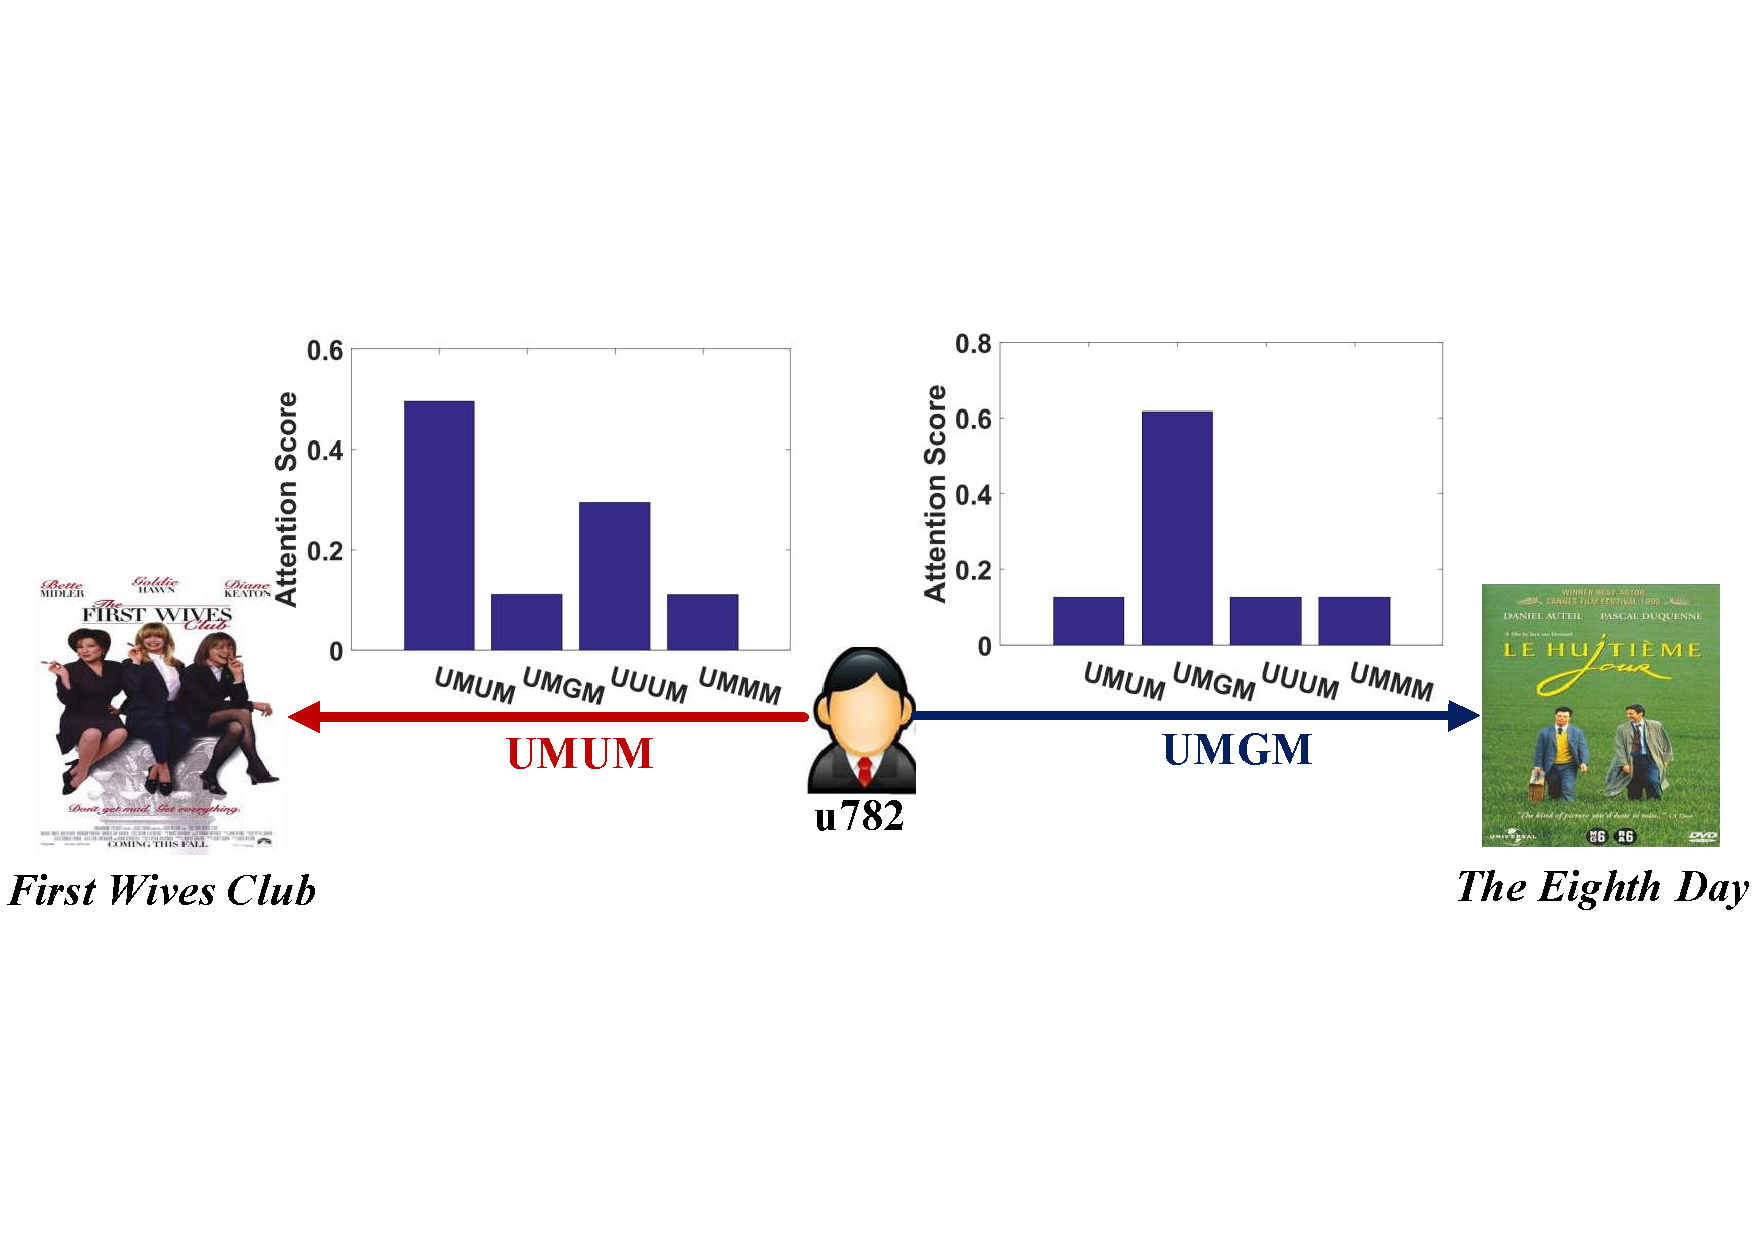
\includegraphics[width=8.5cm]{image/cs_782_2.pdf}\\
  \caption{An illustrative example of the interpretability of interaction-specific attention distributions for MCRec.  \label{fig-casestudy}}
\end{figure}


To see this, we select the user $u782$ in the Movielens dataset as an illustrative example. Two interaction records of  this user have been used here, namely movies of ``\emph{First Wives Club}'' and ``\emph{The Eighth Day}''. In Fig.~\ref{fig-casestudy}, we can see that each interaction corresponds to a unique attention distribution, summarizing the contributions of the meta-paths. The first interaction mainly relies on the meta-paths of $UMUM$ and $UUUM$, while the second interaction mainly relies on the meta-path of $UMGM$. By inspecting into the dataset, it is found that at least five friends of $u782$ have watched the movie of ``\emph{First Wives Club}'', which explains why user-oriented meta-paths  $UMUM$ and $UUUM$ play the key role in the first interaction. As for the second interaction, we find that the movie of ``\emph{The Eighth Day}'' is with the genre of \emph{Drama}, which is the favorite movie genre of $u782$. This explains why genre-oriented meta-path $UMGM$ plays the key role in the second interaction.
Our model is able to produce interaction-specific attention distributions, providing a good interpretability for the recommendation results.

%Furthermore, we investigate the attention scores and recommendations of a concrete user. We select the user $u782$ in the Movielens dataset, and report the distribution of attention scores of this user and the movies recommended in the Fig.~\ref{fig-casestudy}. When recommending the movie ``The Eighth Day'', we find the meta-path $UMGM$ plays the leading role. When we analyze the view records of this user, we can find the favorite of this user are genre Drama, Comedy and Thriller, and the recommended movie ``The Eighth Day'' is just Drama. Meanwhile, the meta-path $UMUM$ is more important when recommending the movie ``First Wives Club''. A potential reason is that the movie ``First Wives Club'' is often watched by users having the same viewing records with the user $u782$, that is the truth after we analyzed the data.  The above analysis reflects that the attention scores of meta-paths effectively reveal users' preferences and the path semantics are potential for explanation recommendation.

After examining how the co-attention works at the user level, we further present the macro-level analysis of the attention distributions for the entire dataset.
We present the box-plot figure of the attention weight distributions from all the interaction records of a dataset in Fig.~\ref{fig-attention-distribution}.
We can see that  the distributions of attention weights are indeed very skew,  indicating some meta-paths are more important to consider than the others.
%In this section, we study the reasonability and physical meaning of meta-paths' attention scores discovered by MCRec. We first make a statistics on the attention scores in the above experiments, and report the distribution of these attention scores in Fig.~\ref{fig-attention-distribution}. As shown in Fig.~\ref{fig-attention-distribution}, we can find that users in the Movielens dataset prefer the meta-path $UMGM$, while users in the Yelp dataset prefer the meta-path $UBCaB$ and $UBCiB$. However, in the LastFM dataset, the distribution of attention scores on each meta-path is quite close. It reveals that the meta-paths in the LastFM dataset have similar contribution on recommendation.  We think it is also the reason why the performance improvement of MCRec against MCRec$_avg$ is not much significant in the Table~\ref{tab_Effectiveness}.

\begin{figure*}[htbp]
\centering
\subfigure[Movielens]{
\begin{minipage}[t]{0.3\linewidth}
\centering
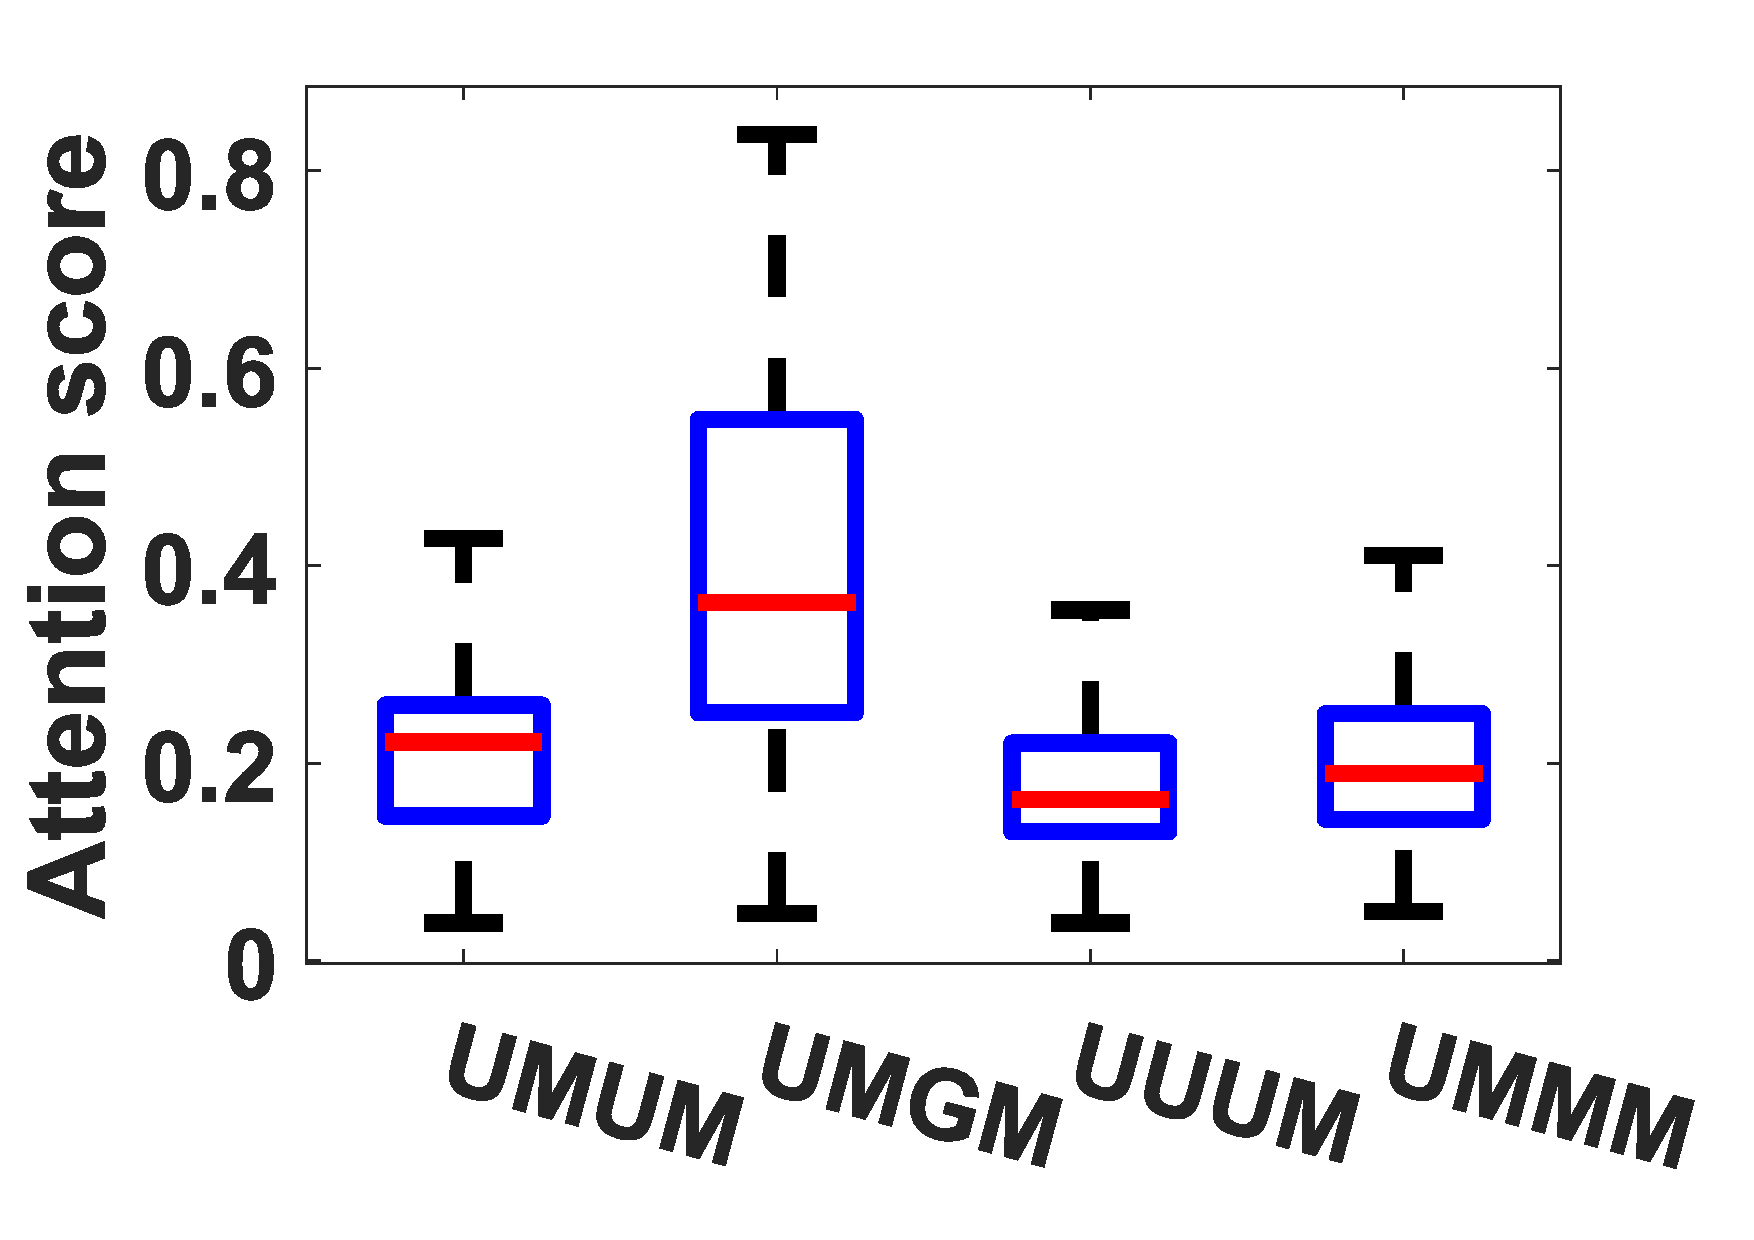
\includegraphics[width=4.2cm]{image/ml_attention_box.pdf} %2.8
\end{minipage}
}
\subfigure[LastFM]{
\begin{minipage}[t]{0.3\linewidth}
\centering
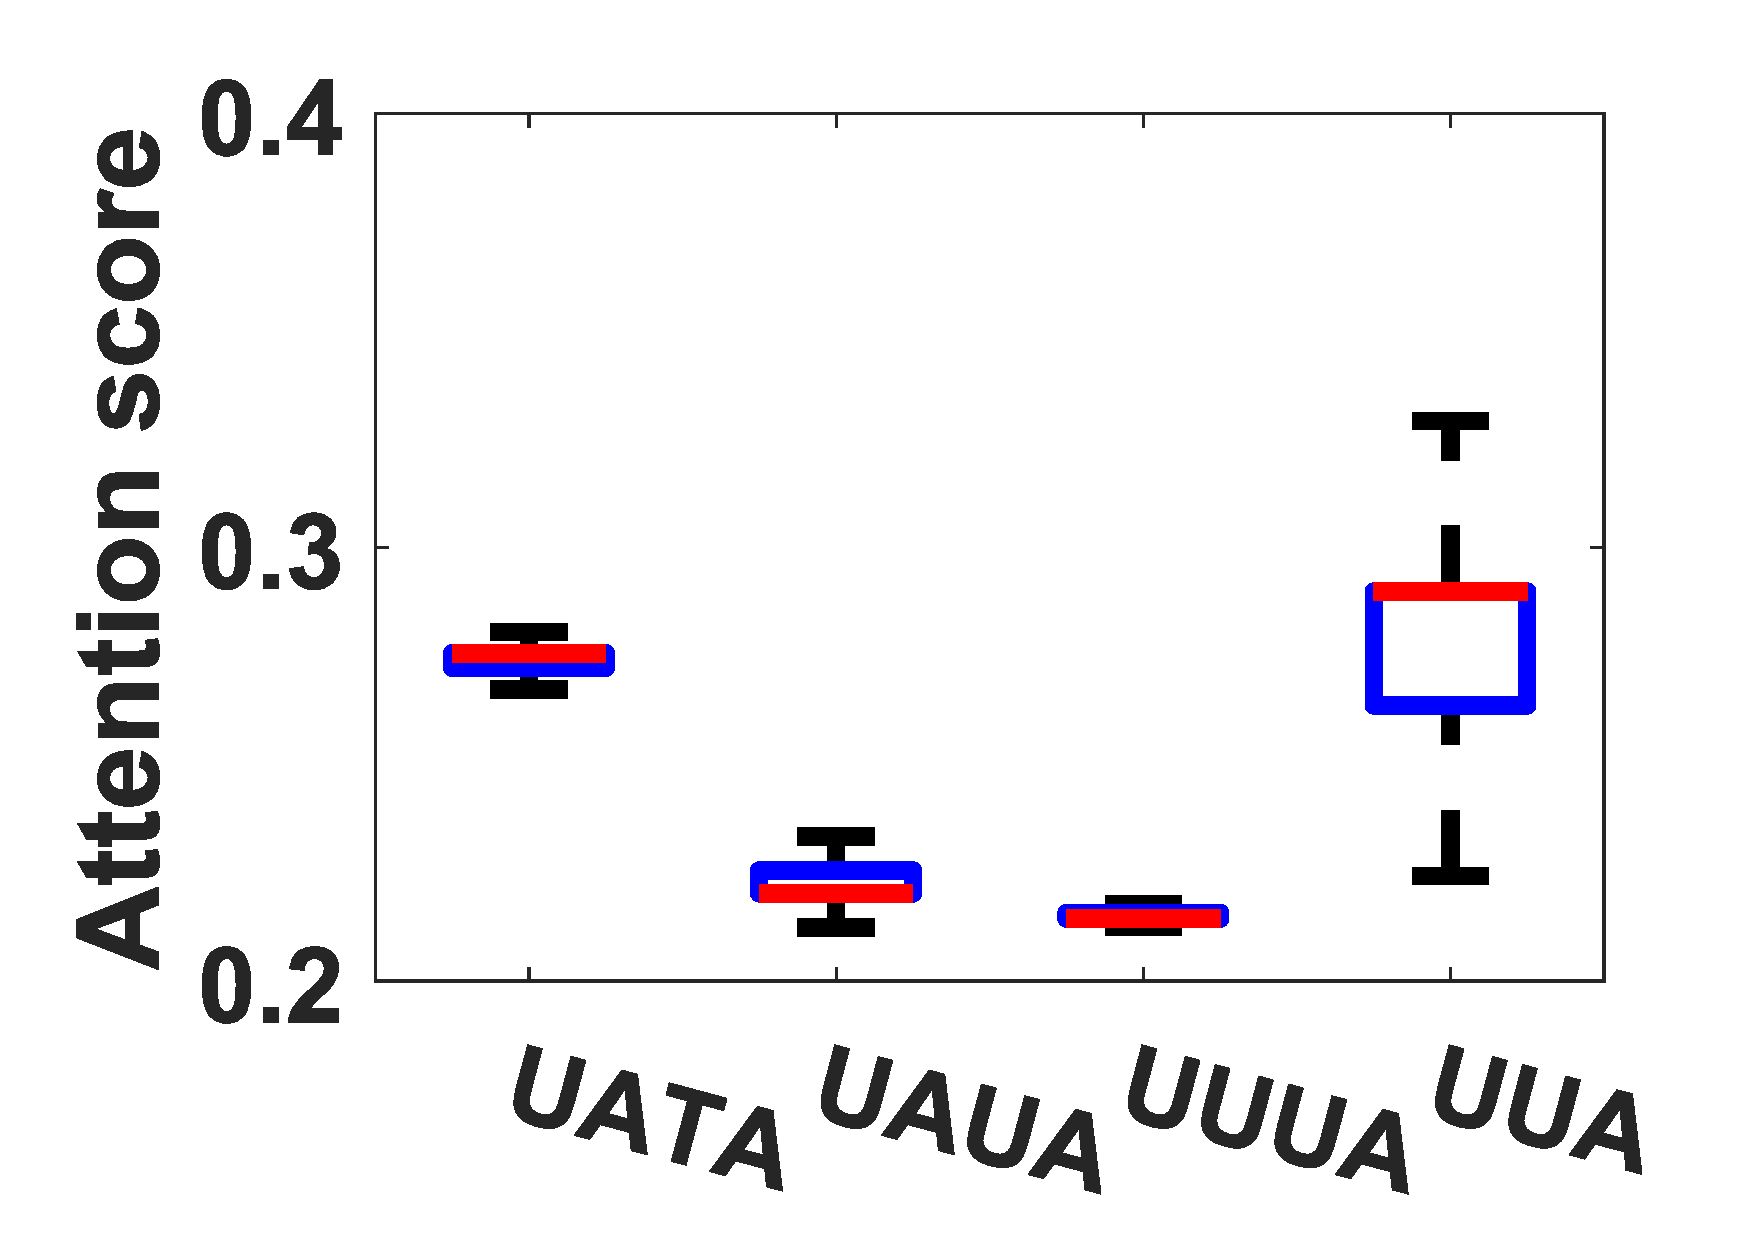
\includegraphics[width=4cm]{image/lm_attention_box.pdf} %2.6
\end{minipage}
}
\subfigure[Yelp]{
\begin{minipage}[t]{0.3\linewidth}
\centering
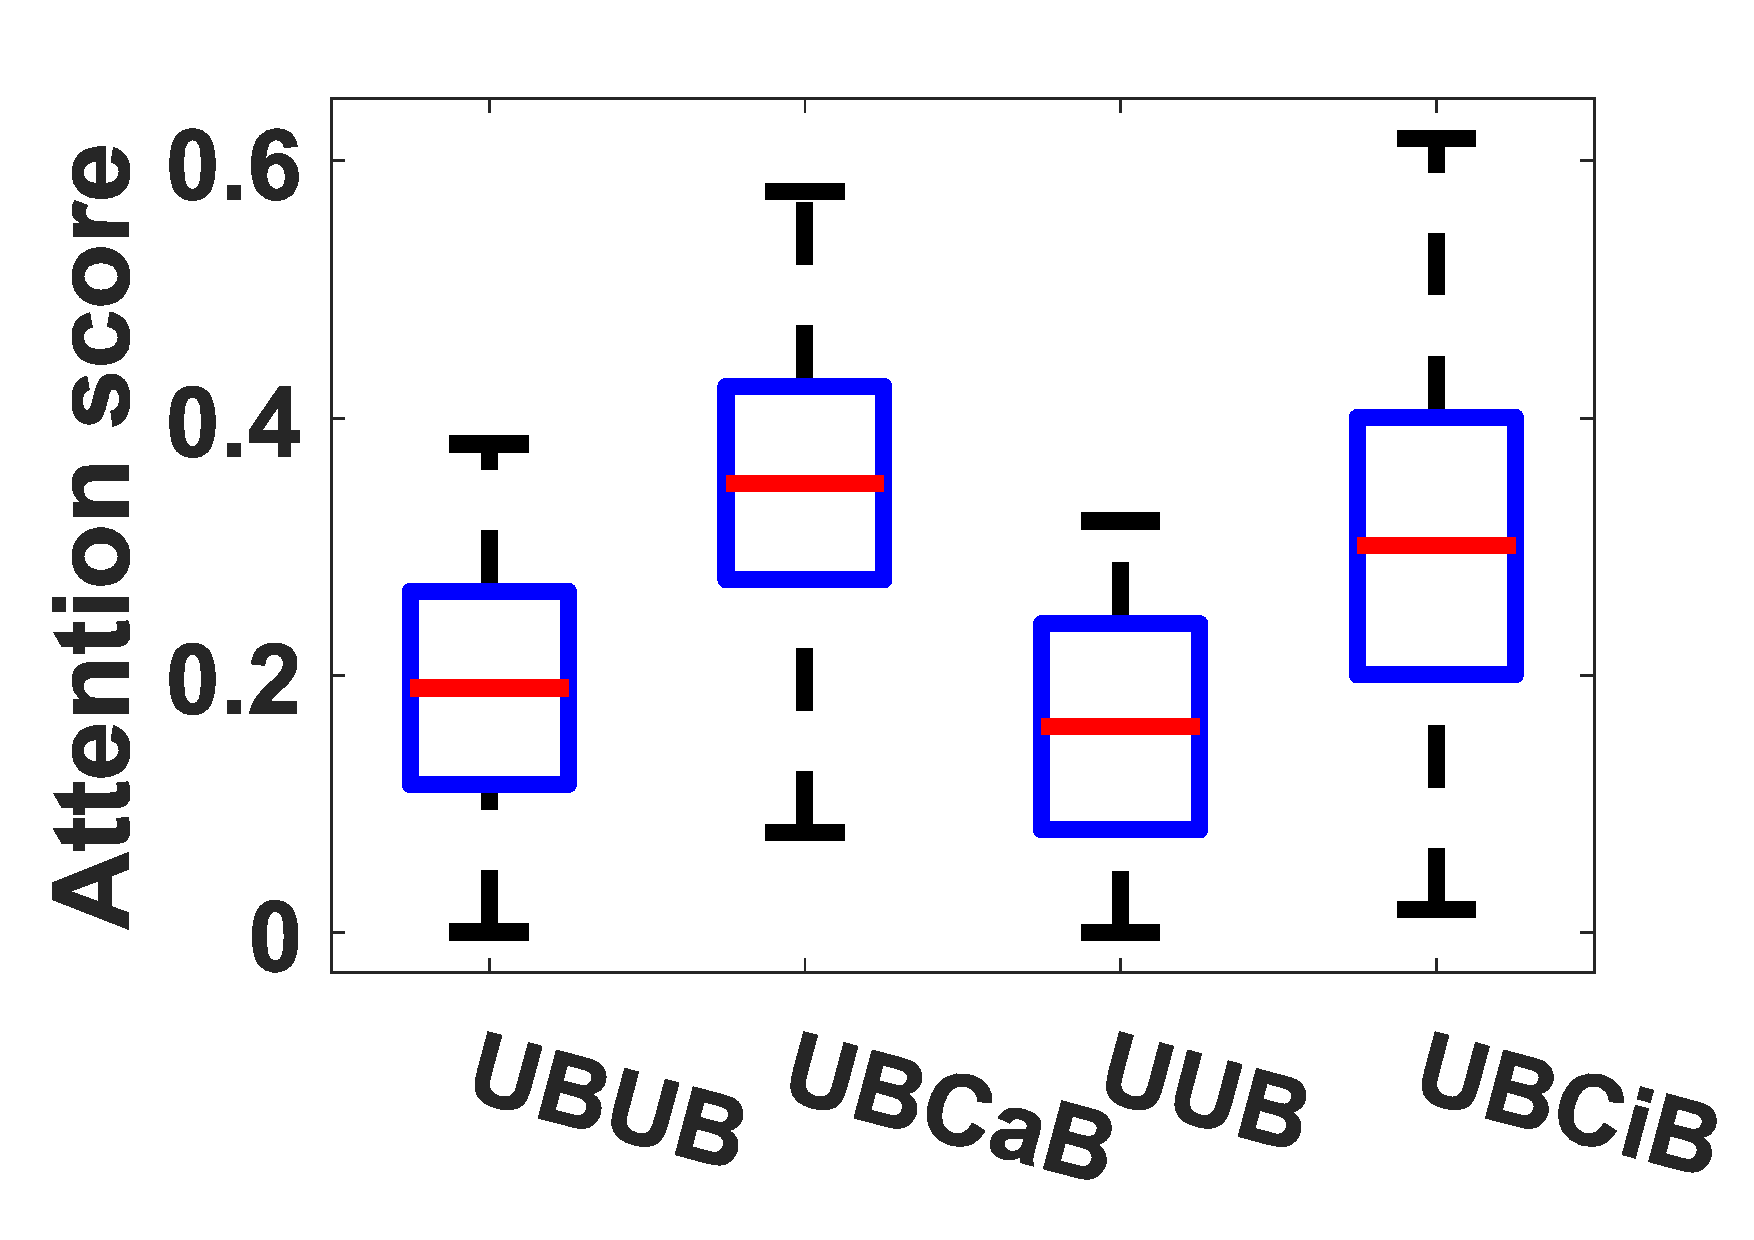
\includegraphics[width=4.2cm]{image/yelp_attention_box.pdf} %2.8
\end{minipage}
}
\caption{The distribution of attention weights of MCRec on the three datasets. \label{fig-attention-distribution}}
\end{figure*}


\subsubsection{Cold-start Recommendation}
HINs are particularly useful to alleviate  cold-start problem in recommendation, where there are very few rating records but heterogeneous context
information is available. We study the recommendation performance \wrt different cold-start degrees, \ie the feedback sparsity.
We divide the entire dataset into five equal folds. The last fold is held out for test, and then we vary the amount of training data from one fold to four folds, corresponding to 20\%, 40\%, 60\%, 80\% data as training sets.  For comparison, we select three representative baselines: BPR, NeuMF, FMG$_{rank}$.
For convenience, we report the improvement ratios \wrt BPR by other comparison methods. Due to space limit, for the remainder of the paper, we will only show the results from Movielens and Yelp, since LastFM shows similar findings. 
As shown in Fig.~\ref{fig-coldstart}, we can see that MCRec yields the most improvement over BPR in all the cases. Overall, the improvement ratios decrease with the increasing of training data. The results indicate that HIN based information is effective to improve the recommendation performance, and the proposed MCRec method can effectively utilize heterogeneous information in a more principled way.


%We present the performance comparison of different methods in Fig.~\ref{fig-coldstart}. For convenience, we report the improvement ratios \wrt BPR. Overall, most of the comparison methods are better than BPR (\eg a positive y-axis value). The proposed method performs the best among all the methods, and the improvement over BPR becomes more significant for users with fewer rating records. The results indicate that HIN-based information is effective to improve the recommendation performance, and the proposed MCRec method can effectively utilize heterogeneous information in a more principled way.

\begin{figure}[htbp]
\centering
\subfigure[Movielens]{
\begin{minipage}[t]{0.45\linewidth}
\centering
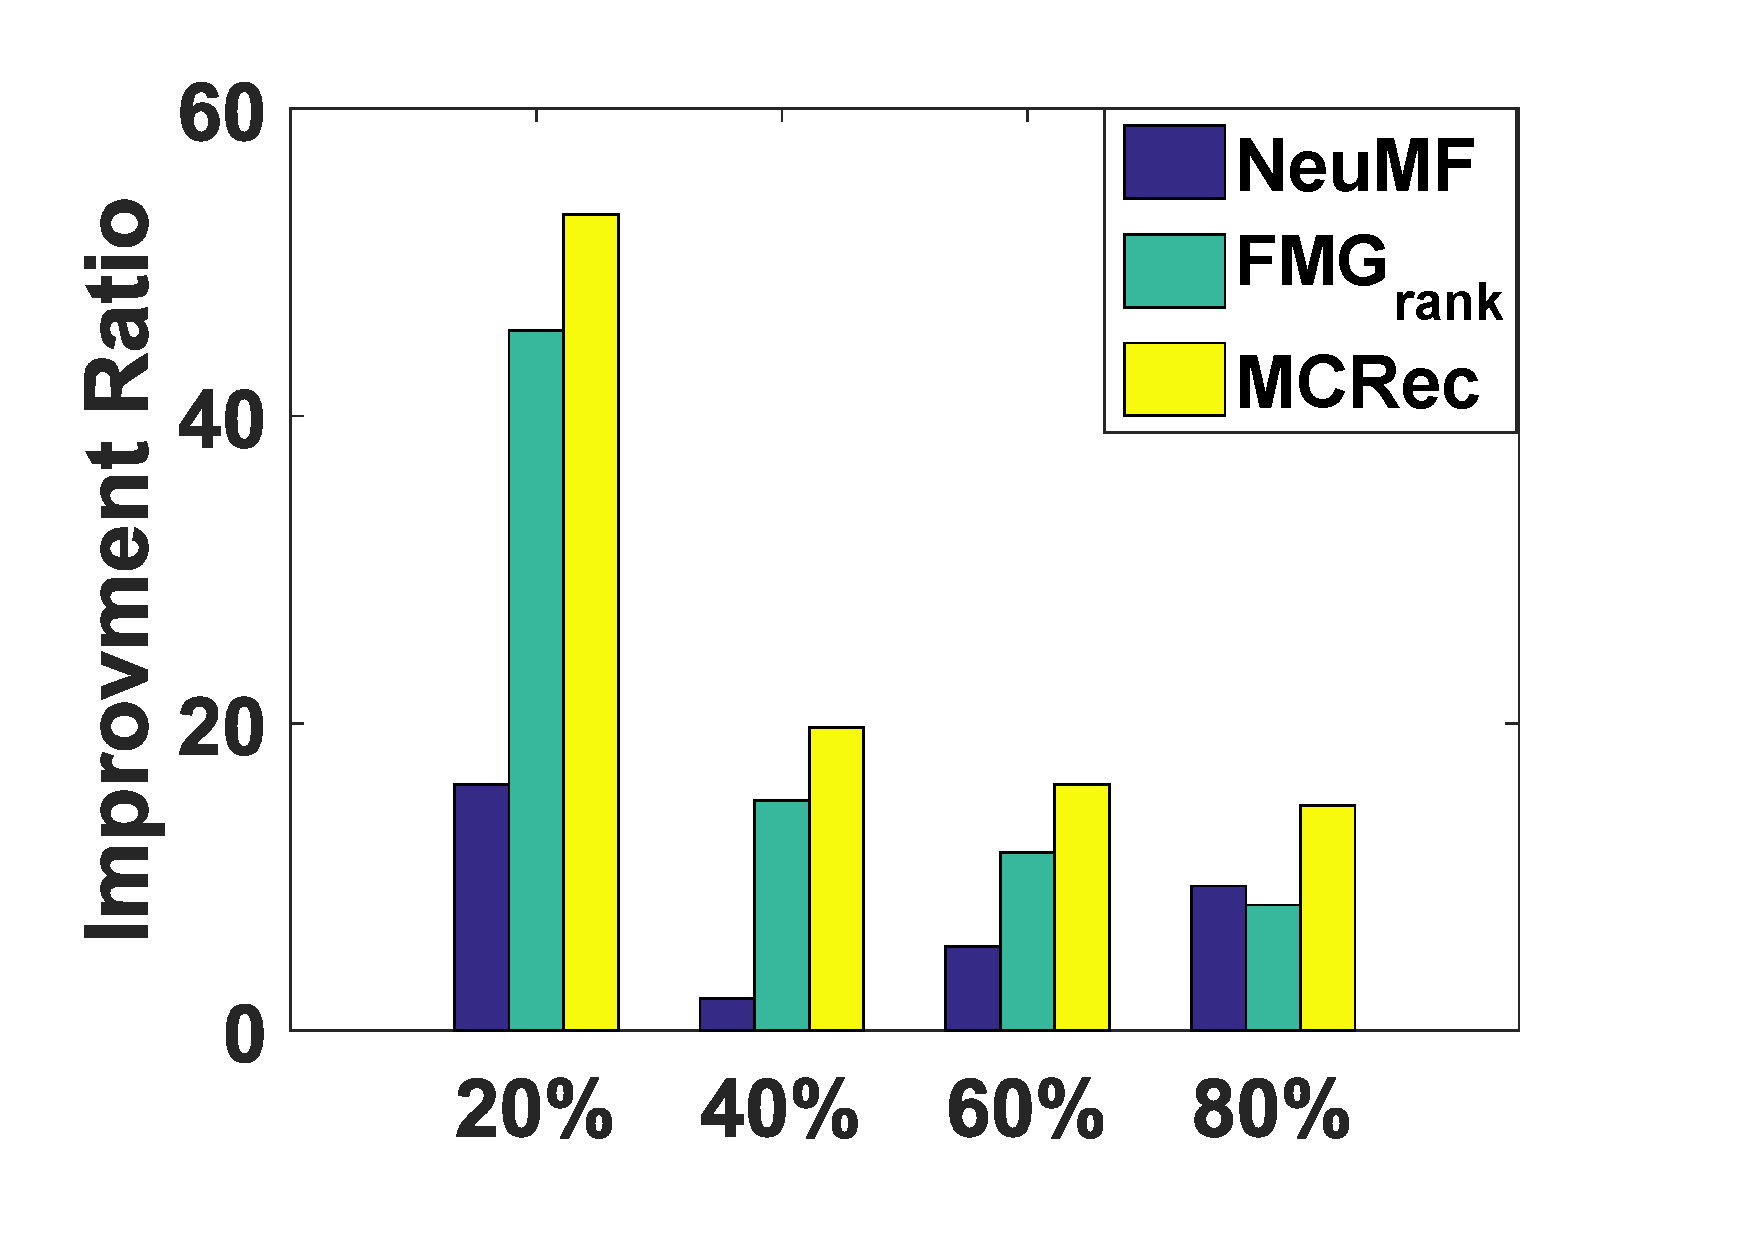
\includegraphics[width=4.4cm]{image/ml_coldstart.pdf}
\end{minipage}
}
%\hspace{30pt}
\subfigure[Yelp]{
\begin{minipage}[t]{0.45\linewidth}
\centering
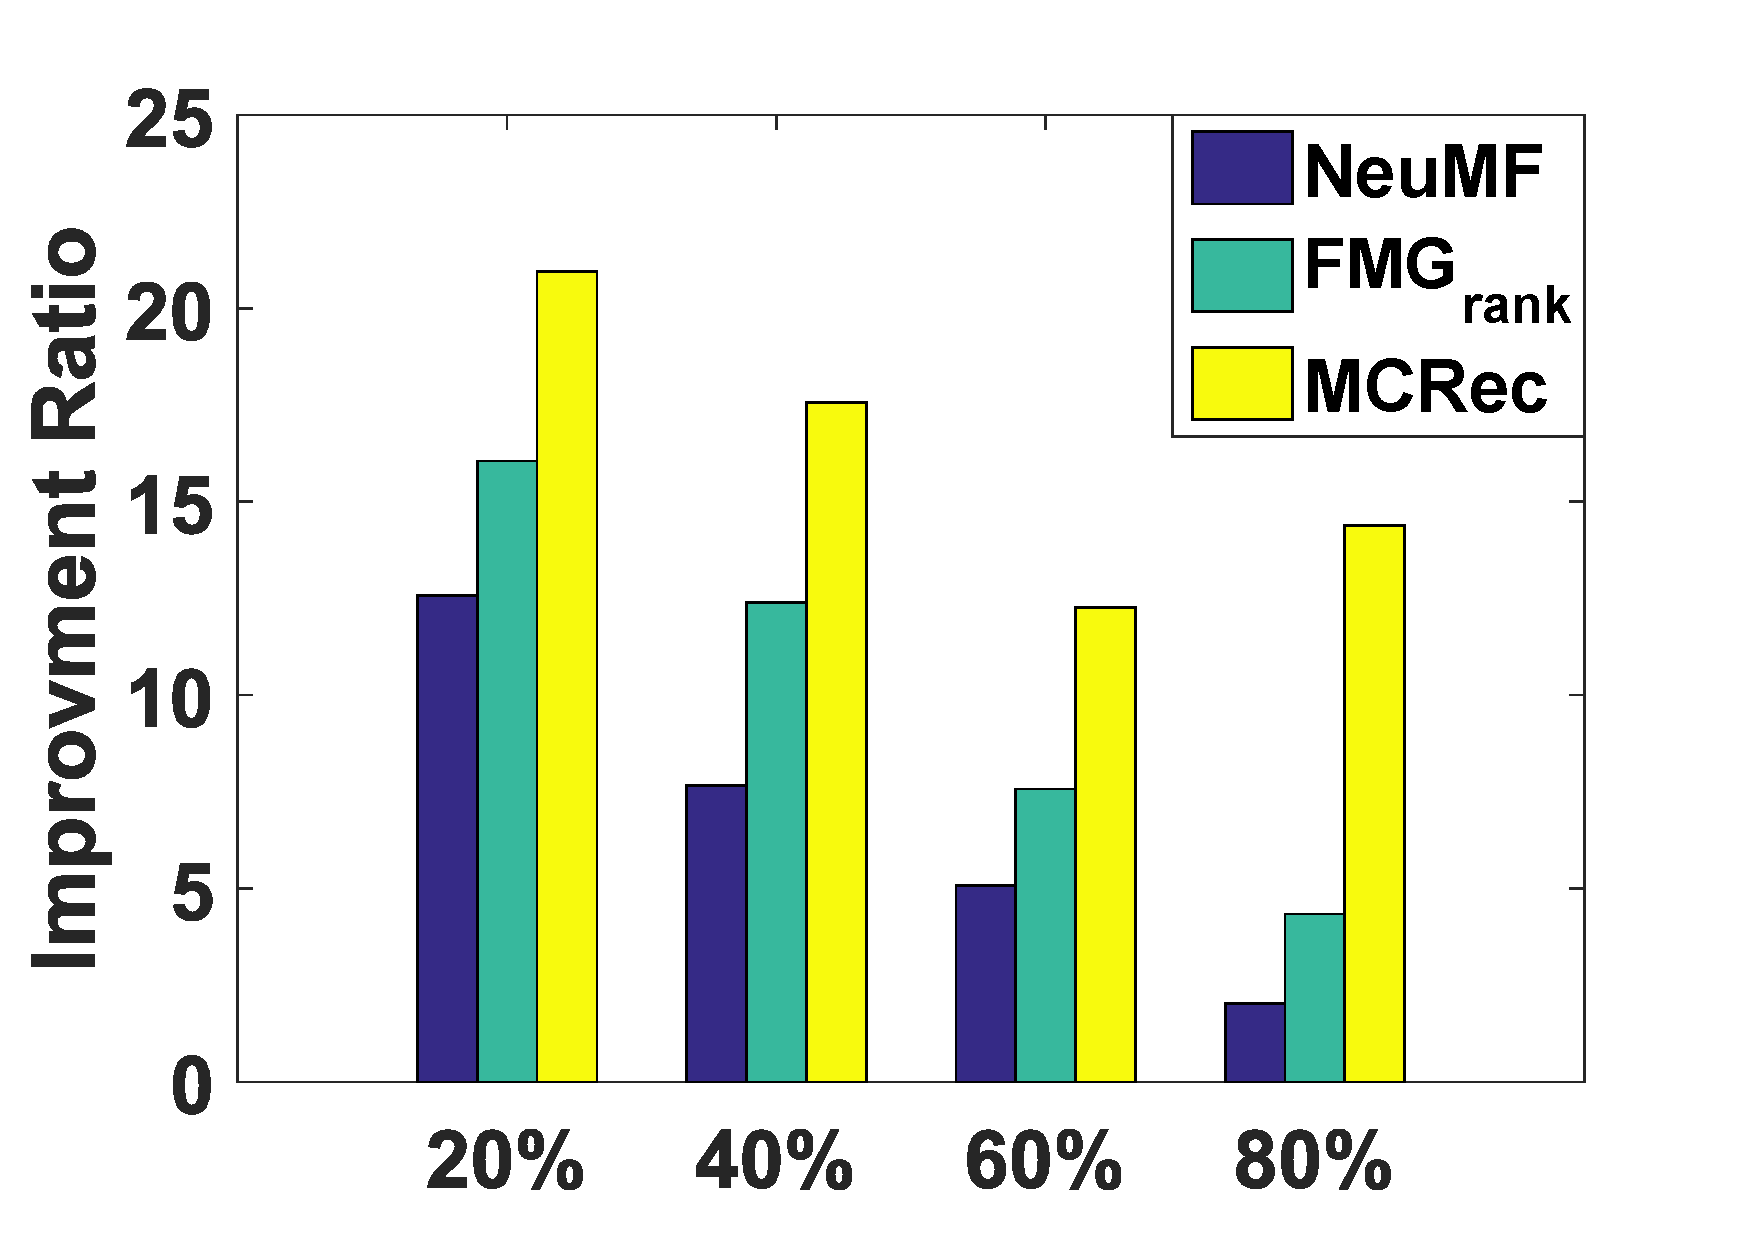
\includegraphics[width=4.3cm]{image/yelp_coldstart.pdf}
\end{minipage}
}
\caption{Performance comparison of different methods for cold-start recommendation on Movielens and Yelp datasets. $y$-axis denotes the improvement ratio over BPR for $Prec@10$.\label{fig-coldstart}}
\end{figure}



\subsubsection{Impact of Different Meta-Paths}
In this section, we analyze the impact of different meta-paths on the recommendation performance through gradually incorporating meta-paths into the proposed model. For ease of analysis, we include the NeuMF as the reference baseline. In Fig.~\ref{fig-meta-path}, we can observe that  the performance of MCRec overall improves with the incorporation of more meta-paths. Meanwhile, meta-paths seem to have different effects on the recommendation performance. Particularly, we can find that, when adding $UMGM$, MCRec has a significantly performance boost in Movielens dataset, while adding $UBCaB$ and $UBCiB$ is more important for Yelp dataset. These findings are consistent with previous observations for attention weights distributions of meta-paths in Fig.~\ref{fig-attention-distribution}, where these meta-paths have higher attention scores.
%We think the reason lies in that these meta-paths contain more useful information for recommendations. Furthermore, we think the same reason makes these meta-paths have larger attention scores in Figure~\ref{fig-attention-distribution}.

\begin{figure}[htbp]
\centering
\subfigure[Movielens]{
\begin{minipage}[t]{0.45\linewidth}
%\centering
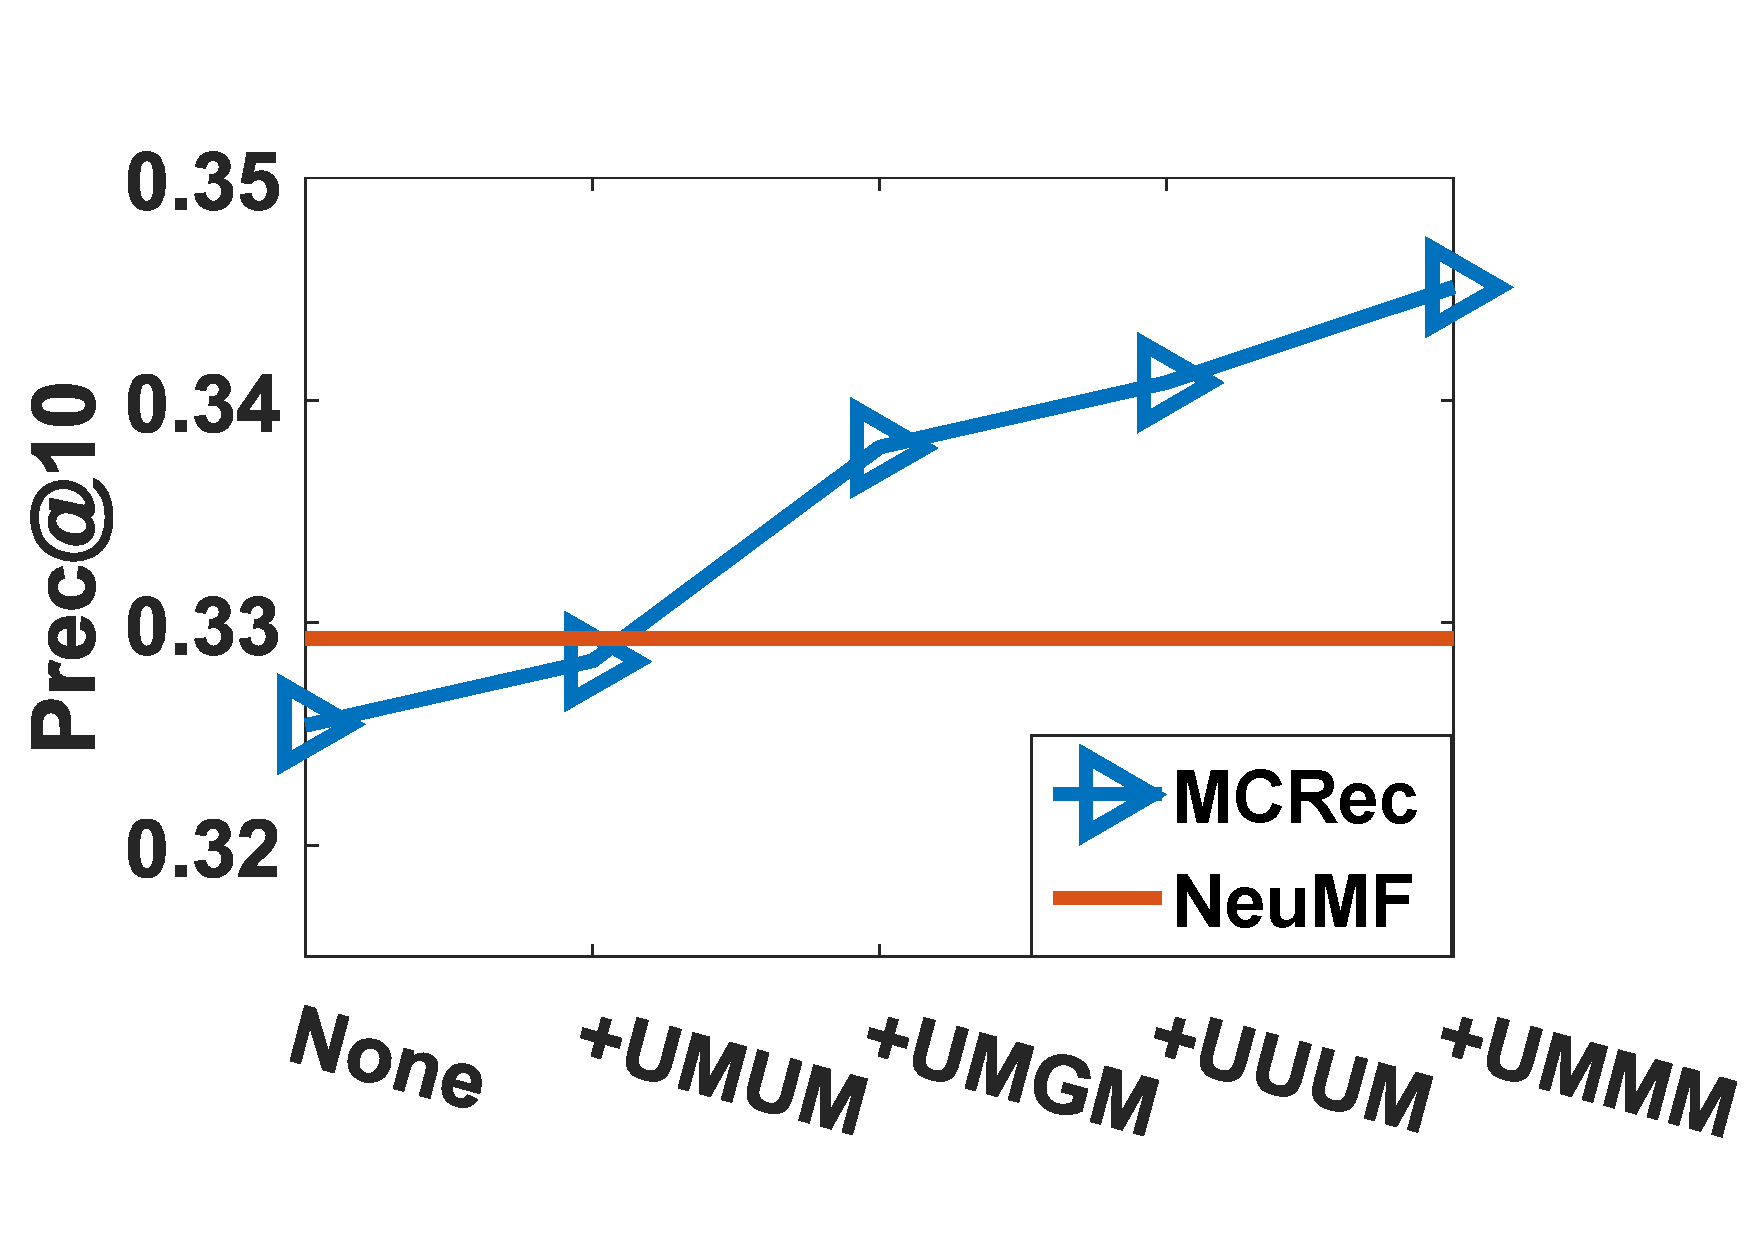
\includegraphics[width=4.15cm]{image/ml_metapath_p.pdf}
\end{minipage}
}
%\hspace{40pt}
\subfigure[Yelp]{
\begin{minipage}[t]{0.45\linewidth}
\centering
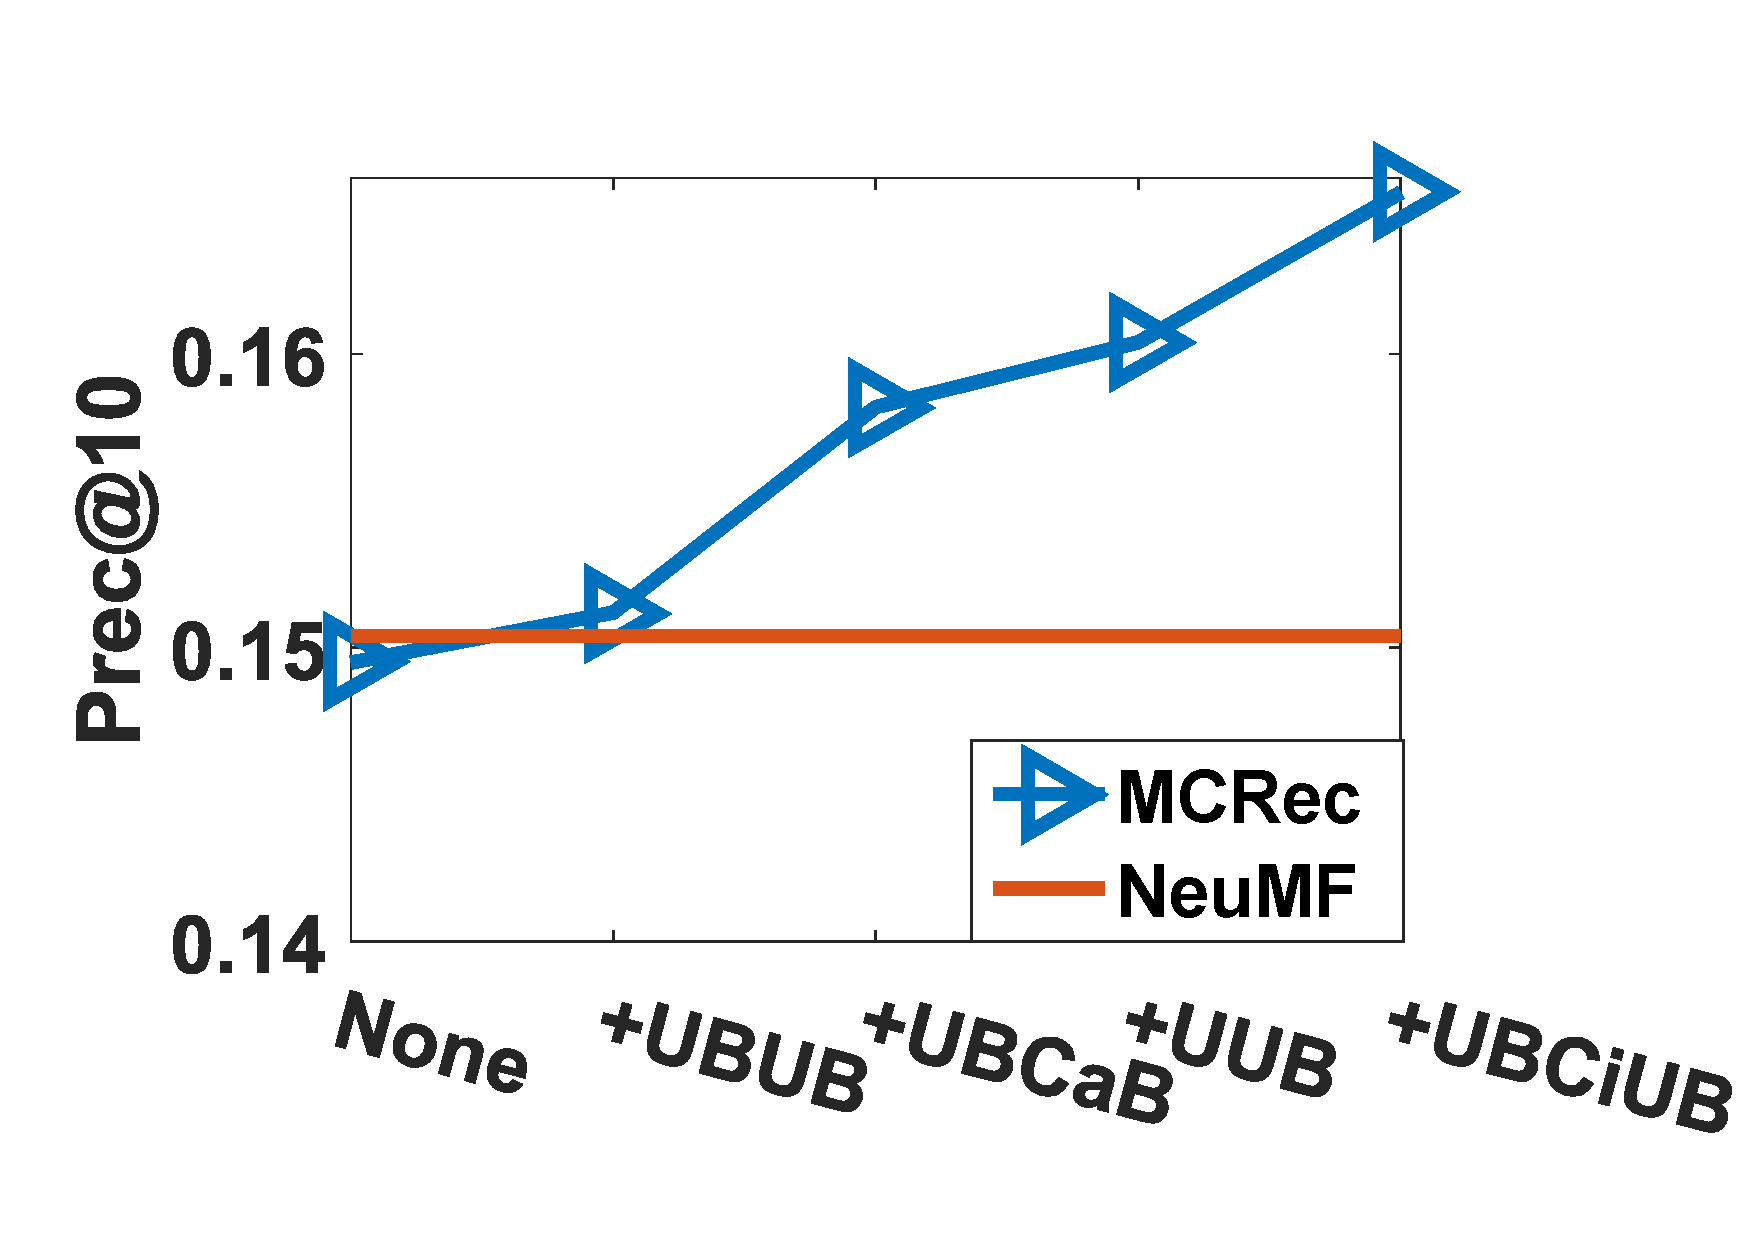
\includegraphics[width=4.2cm]{image/yelp_metapath_p.pdf}
\end{minipage}
}
\caption{Performance change of MCRec when gradually incorporating meta-paths.\label{fig-meta-path}}
\end{figure}


%\subsubsection{Impact of Path Sampling Strategy}
%In Section 4.3.1, we present an importance-based random walk strategy based on meta-path in MCRec. We use the pretrain technique with Factorization Machine to select path instances with higher importance scores. Here, we examine the effectiveness of the propose path sampling strategy.
%In Fig.~\ref{fig-sample}, we can see that the proposed sampling strategy is consistently better than the previous random sampling method.
%With the pretrain latent factors for computing the importance scores, our sampling strategy is able to discover more high-quality path instances for recommendation.

%In order to furtherly validate the effectiveness of  the preference-guided random walk strategy based on meta-path in MCRec, we compare our strategy with traditional path-based random walk strategy widely used in HIN embedding. The results are shown in Fig.~\ref{fig-sample}. We can find the proposed sample strategy significantly  outperforms the traditional strategy. An possible reason is that  the proposed preference-guided walk strategy can sample high-quality path instances, while traditional walk strategy may introduce much noise.
%\begin{figure}[htbp]
%\centering
%\subfigure[Movielens]{
%\begin{minipage}[t]{0.45\linewidth}
%\centering
%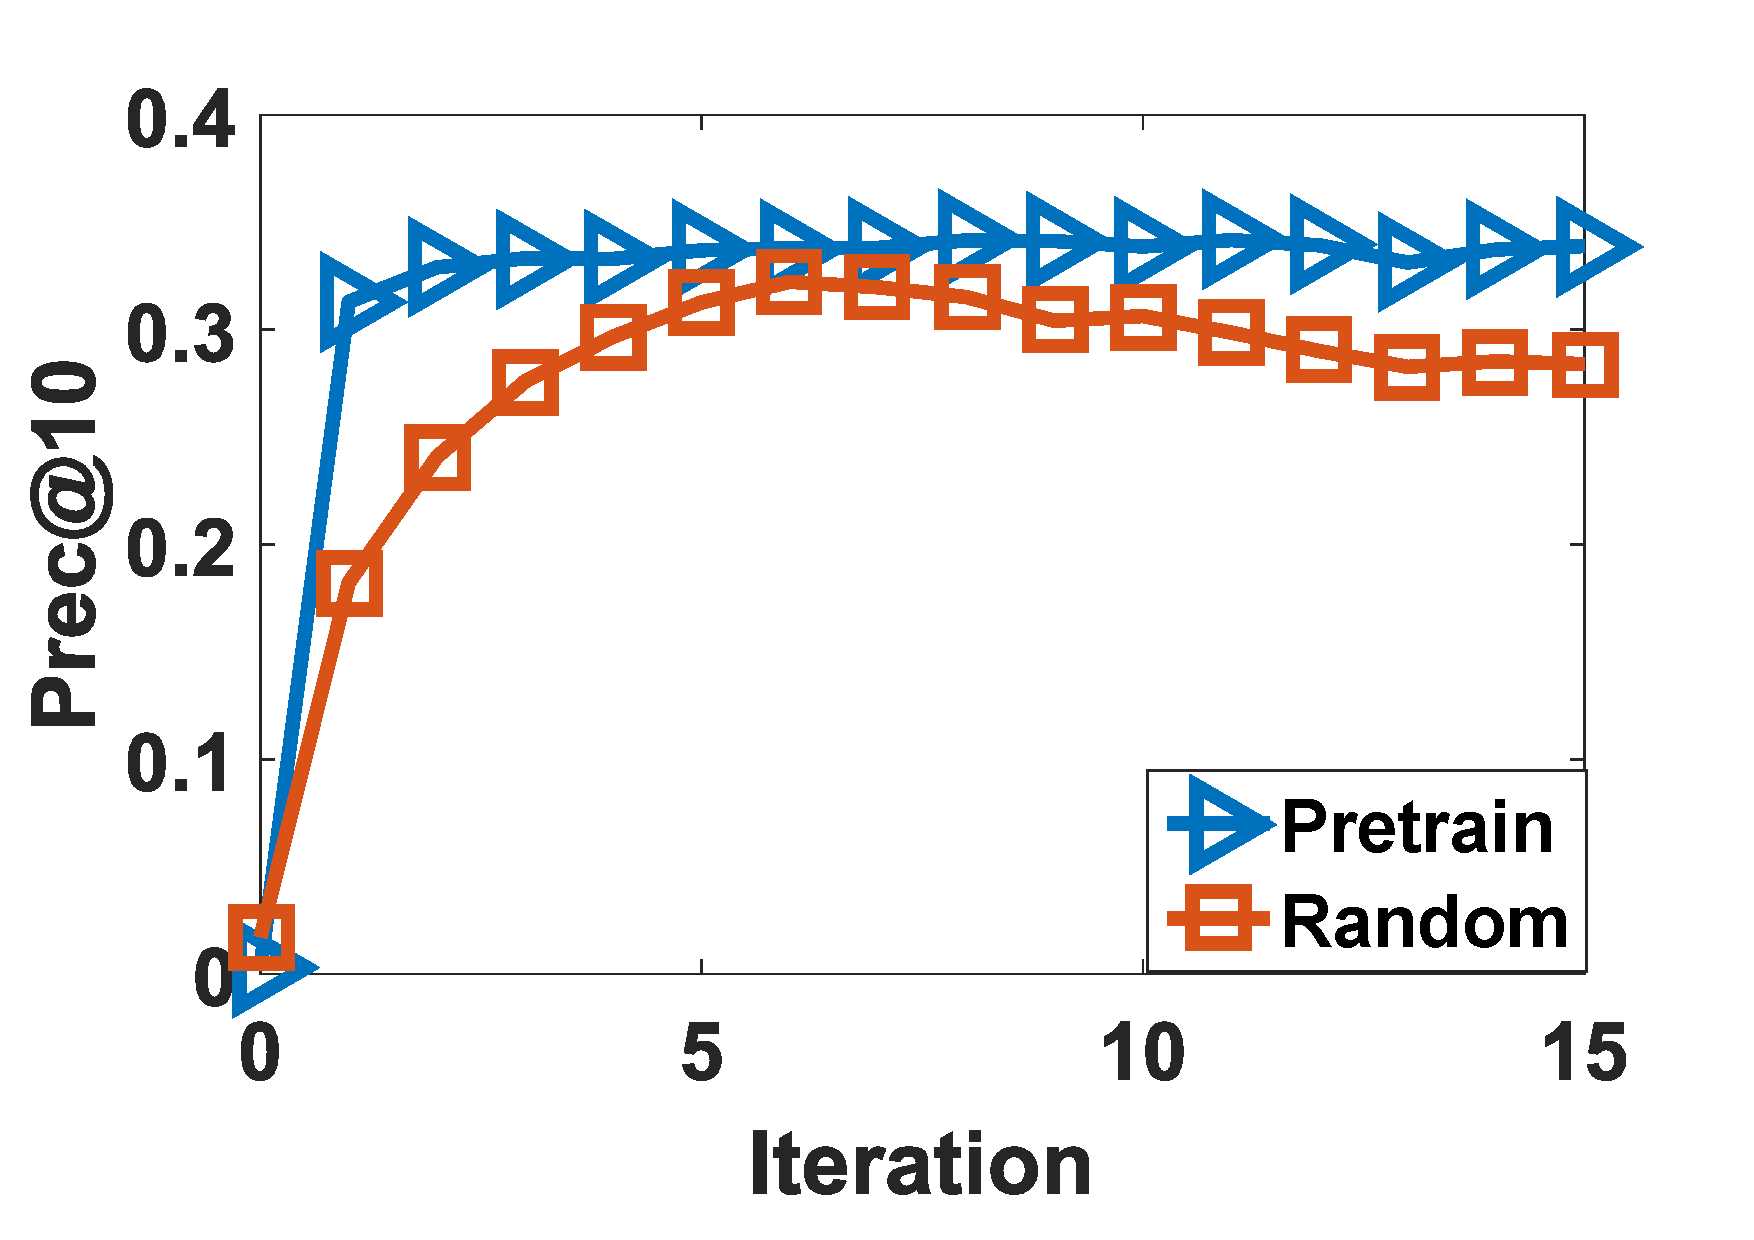
\includegraphics[width=4.2cm]{image/ml_sample_p.pdf}
%\end{minipage}
%}
%\hspace{40pt}
%\subfigure[Yelp]{
%\begin{minipage}[t]{0.45\linewidth}
%\centering
%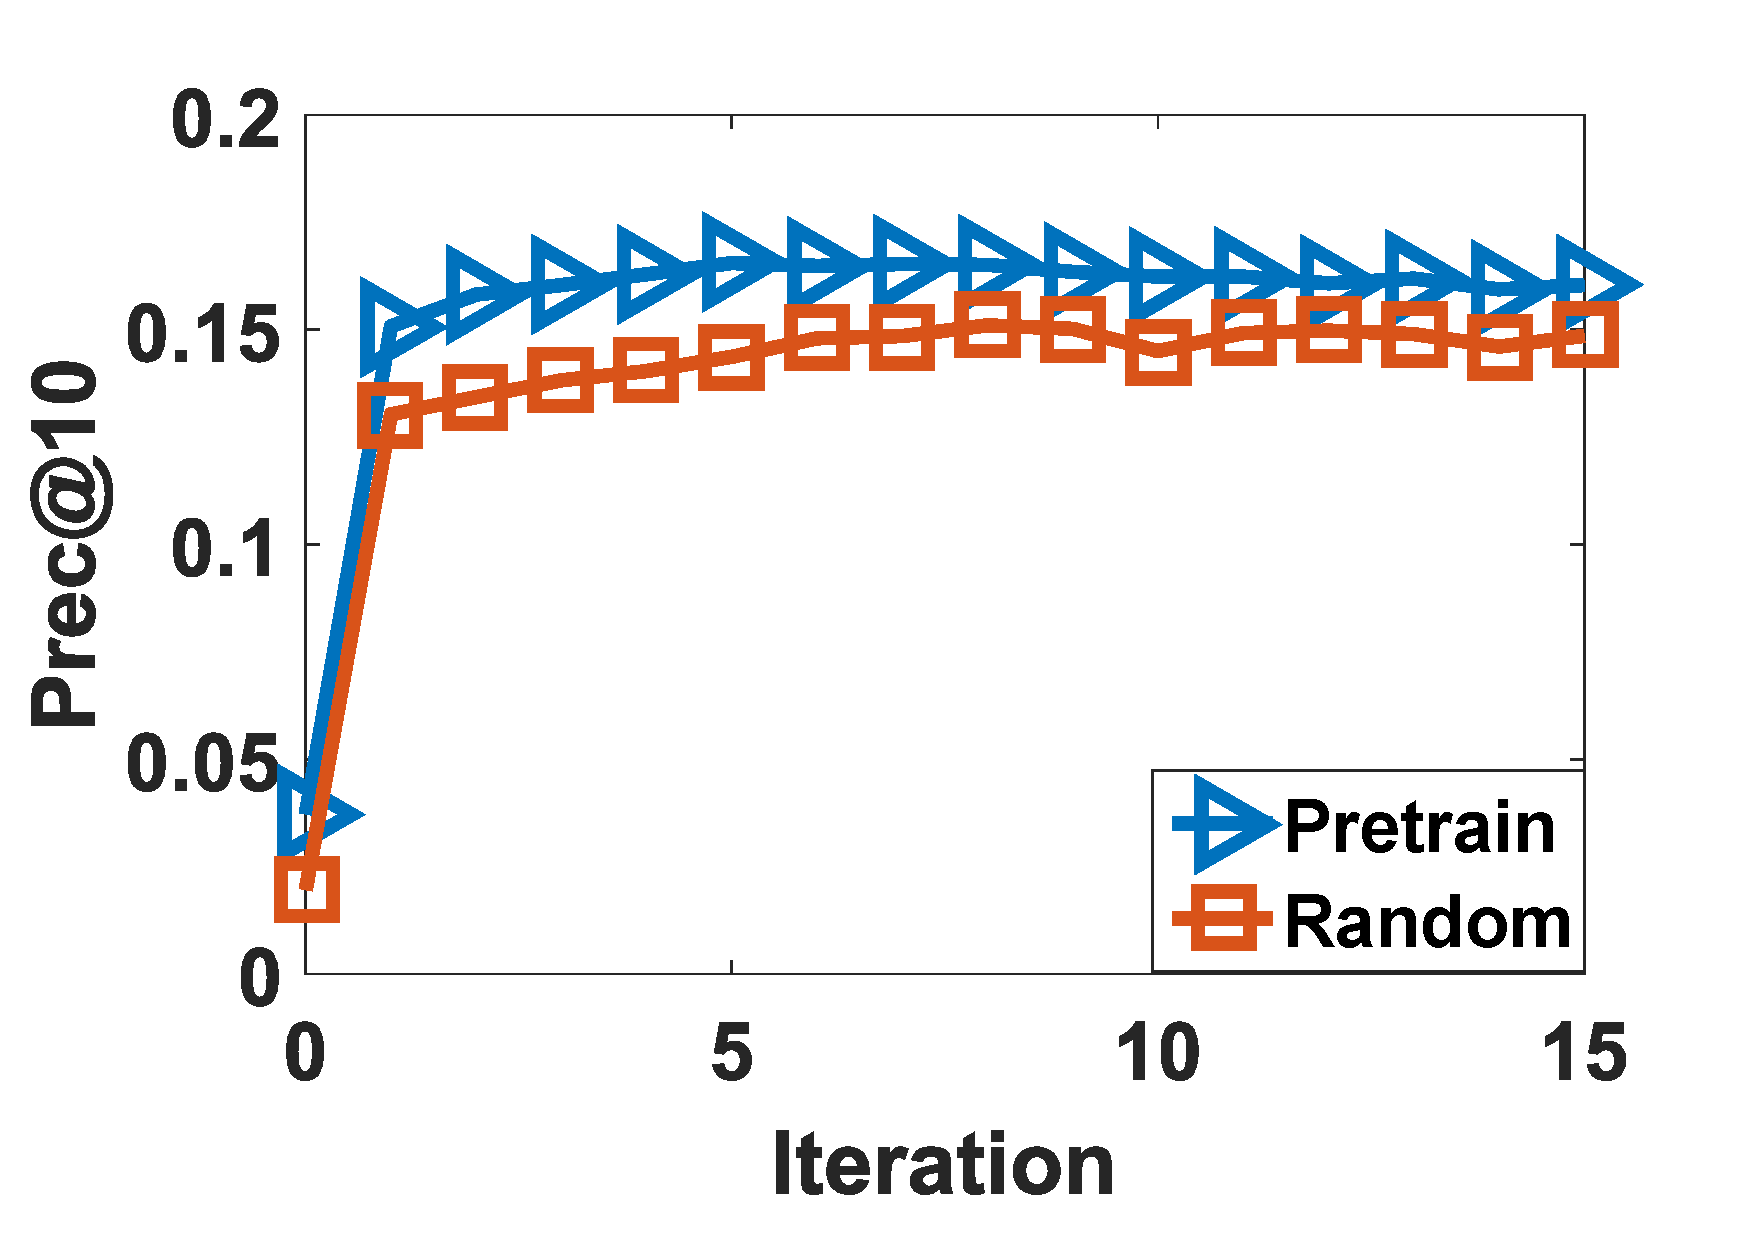
\includegraphics[width=4.2cm]{image/yelp_sample_p.pdf}
%\end{minipage}
%}
%\caption{ Performance with respect to different sampling strategies on Movielens and Yelp datasets.\label{fig-sample}}
%\end{figure}


\subsubsection{Parameter Tuning} Our models include a few important parameters to tune. Here, we examine the performance effect of two parameters, \ie the number of predictive factors (the embedding size for the output layer) and the number of negative samples (in Eq.~\ref{equ-loss}).
For the number of predictive factors, we vary it in the set of \{8, 16, 32, 64\}. For the number of negative samples, we vary it in the set of \{1, 3, 5, 7, 9\}.
As shown in Fig.~\ref{fig-param}, overall MCRec is not sensitive to these two parameters. The optimal performance is obtained with 32 predictive factors and five negative samples.

%near 32. As shown in Fig.~\ref{fig-param}, the optimal performance is around 5.

%In this section, we study two tuning parameters involved in our prediction model, which are the predictive factors and the number of negative samples. Now we check how they influence the model performance. Due to space limitation, we just present the results
%on Movielens dataset.

\begin{figure}[htbp]
\centering
\subfigure[\#predictive factors]{
\begin{minipage}[t]{0.45\linewidth}
\centering
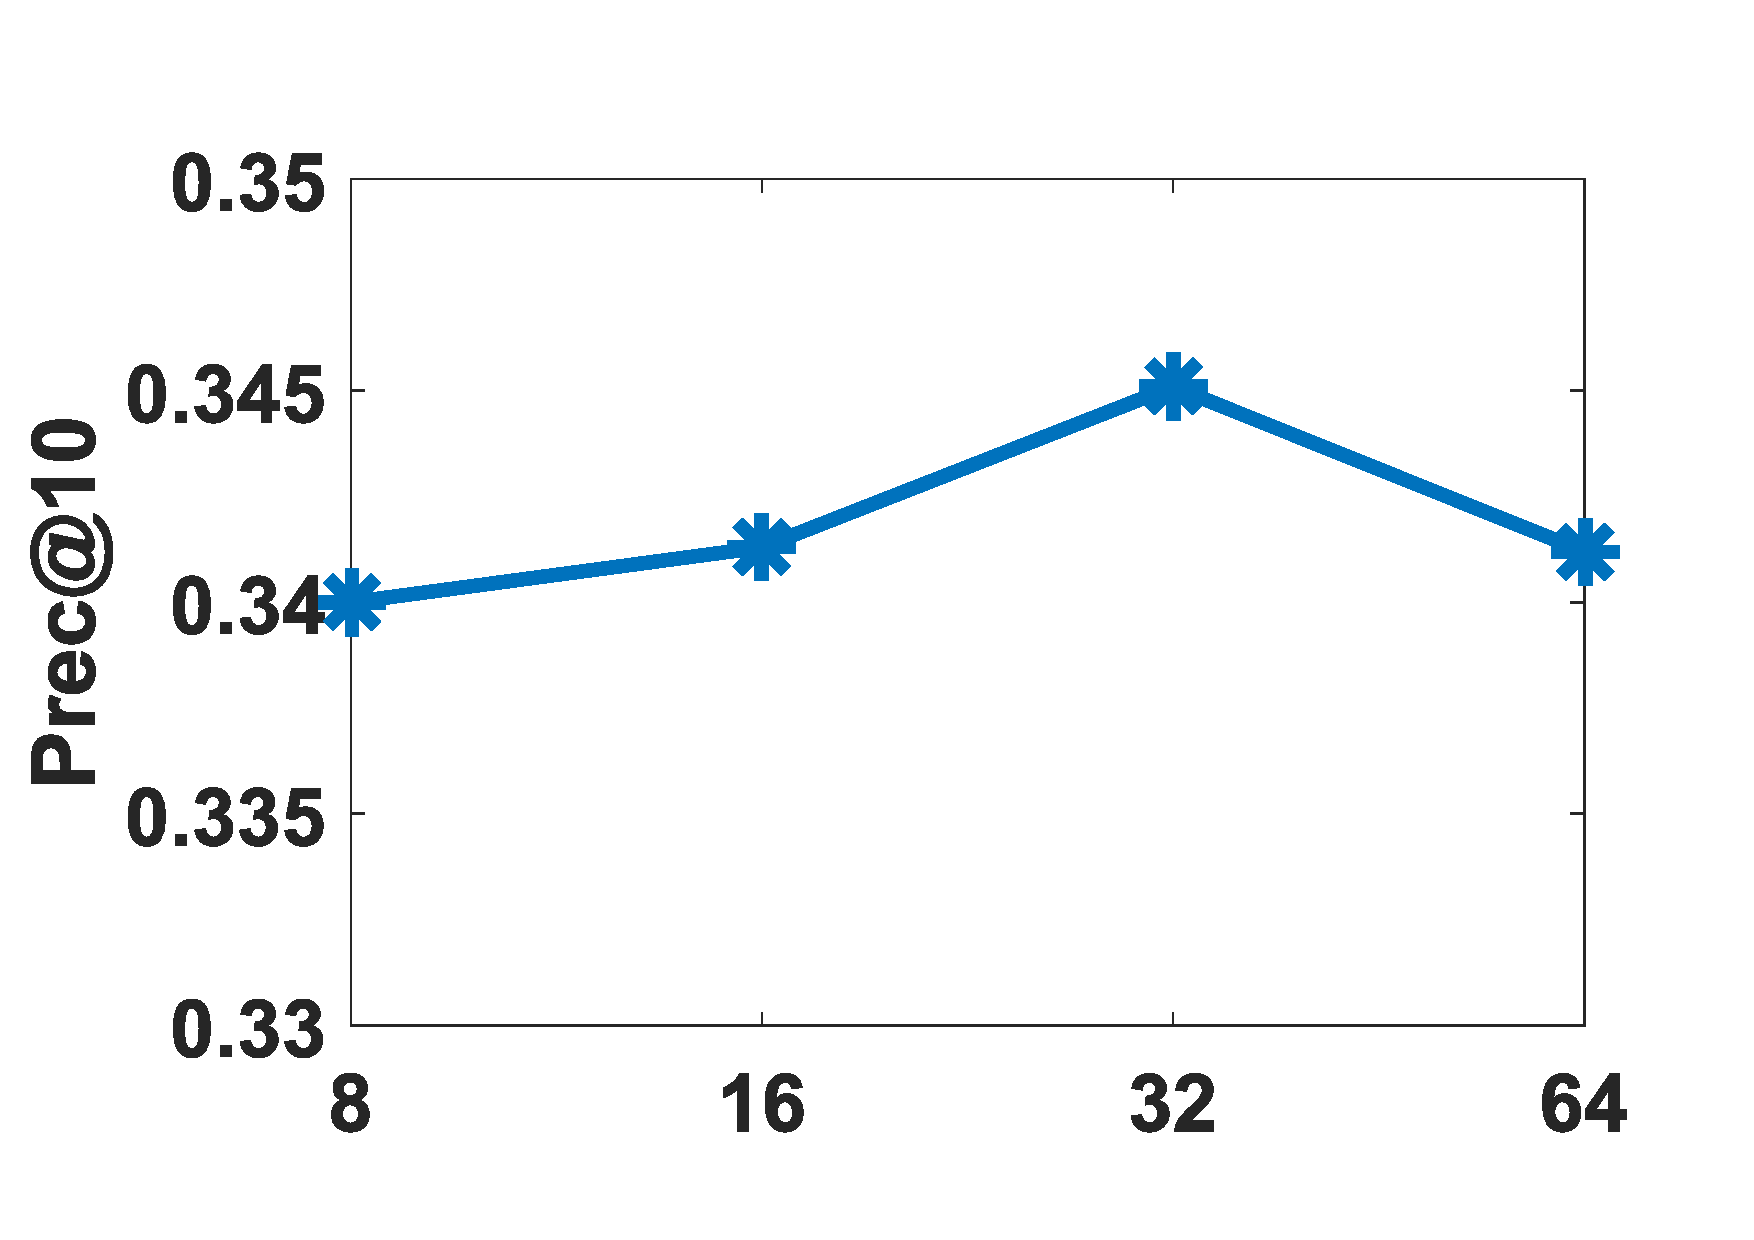
\includegraphics[width=4.2cm]{image/ml_factors_p.pdf}
\end{minipage}
}
%\hspace{40pt}
\subfigure[\#negative samples]{
\begin{minipage}[t]{0.45\linewidth}
\centering
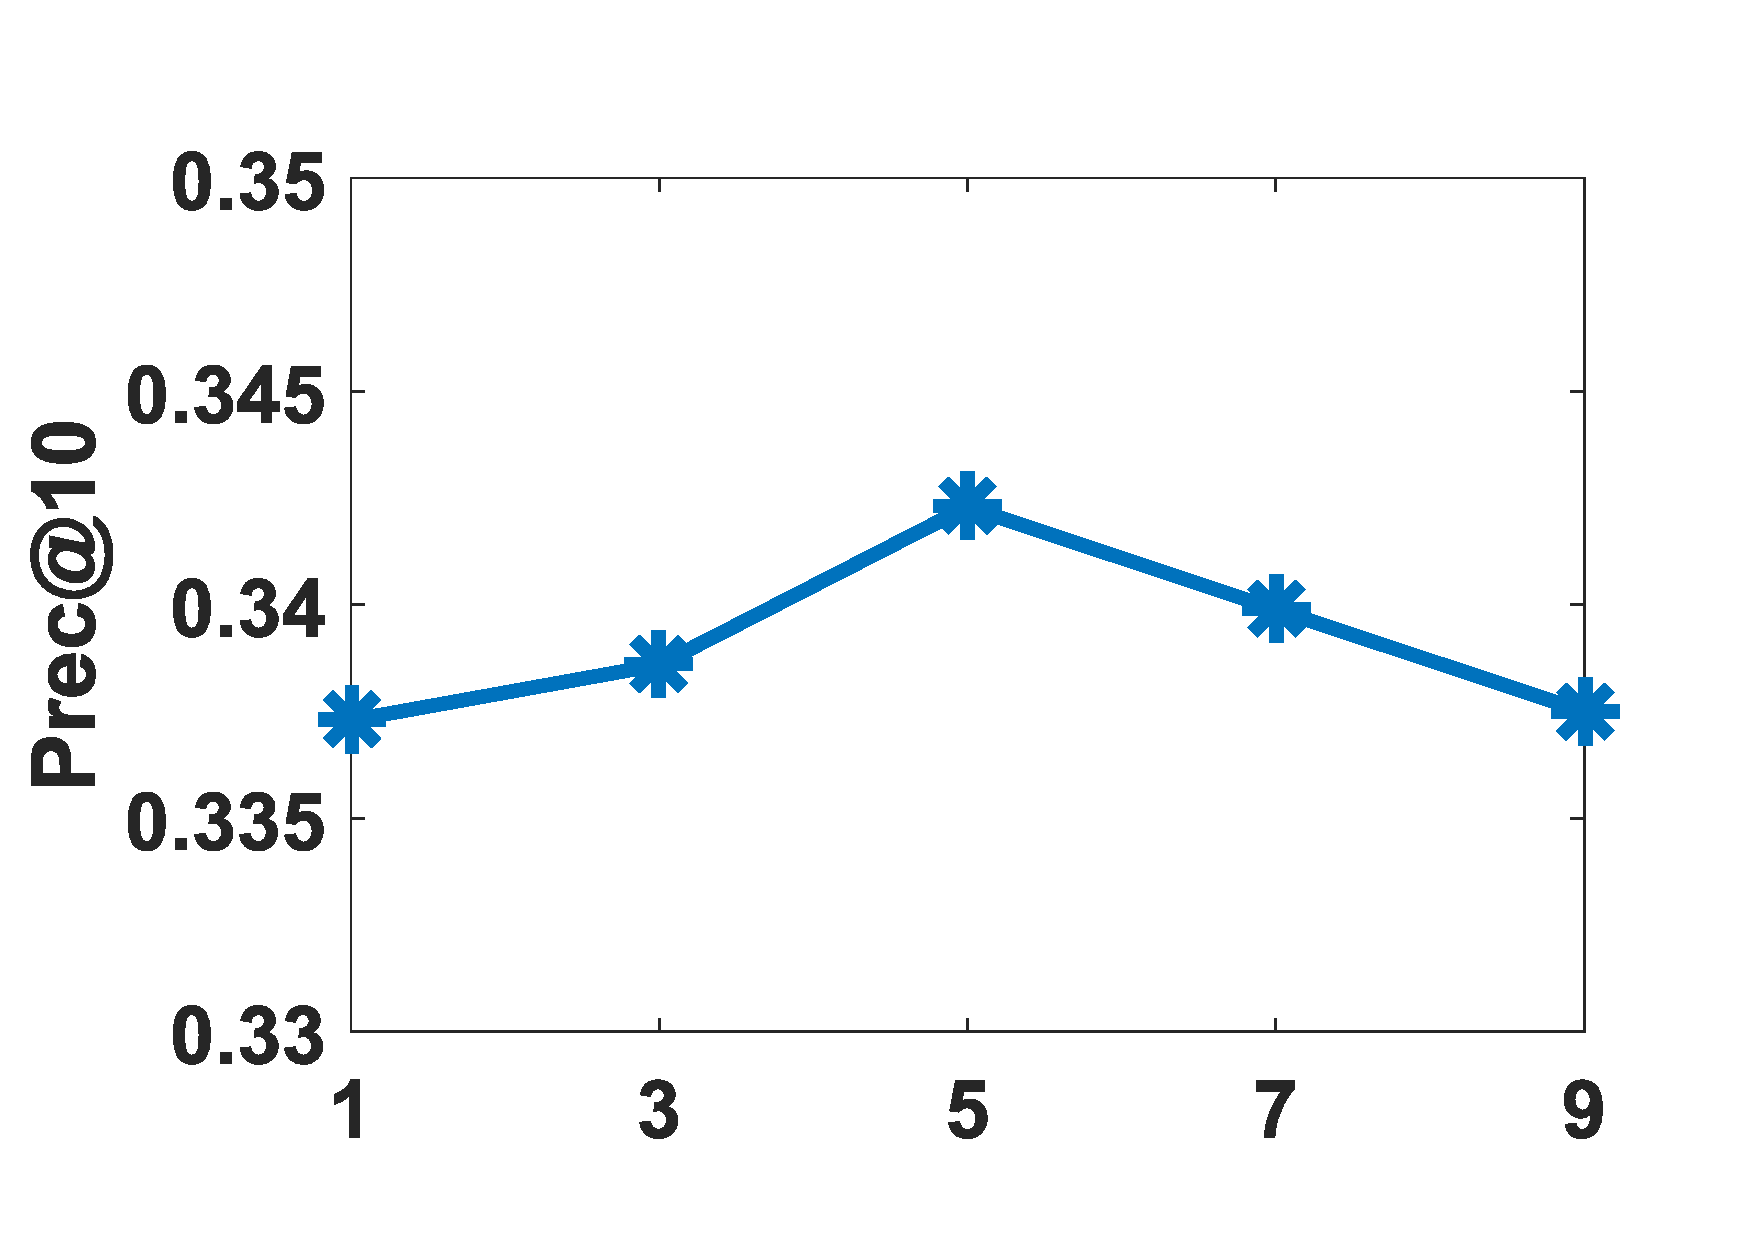
\includegraphics[width=4.2cm]{image/ml_negative_p.pdf}
\end{minipage}
}
\caption{Parameter tuning of MCRec on Movielens dataset.\label{fig-param}}
\end{figure}















\section{Conclusion}

In this paper, we proposed a novel deep neural network model with the co-attention mechanism for top-$N$ recommendation in HIN. 
We elaborately designed a three-way neural interaction model by explicitly incorporating meta-path based context.
 To construct the meta-path based context, we used a priority based sampling technique to select high-quality path instances.
 Our model learned effective representations for users, items and meta-path based context for implementing a powerful interaction function.
The co-attention mechanism  mutually improved the representations for  meta-path based context, users and items. 
Extensive experimental results have demonstrated  the superiority  of our model in both recommendation effectiveness and interpretability. 
We believe the proposed three-way neural interaction model provides a promising approach to utilize HIN information for improving recommender systems. 

Currently, our approach is able to effectively select high-quality path instances, and  learn the attention weights of meta-paths. While, the selection of meta-paths is completed manually.  As future work, we will consider how to develop a more principled way for automatically selecting meta-paths in HINs. We will also consider adapting our approach to deal with more complicated structure patterns in HIN, \eg meta-graphs. In addition, we also will extend our model to deal with explicit feedback as well as weighted edges.

\section{Acknowledgement}
This work is supported in part by the National Natural Science Foundation of China (No. 61772082, 61502502, 61320106006, 61375058), the National Key Research and Development Program of China (2017YFB0803304), and the Beijing Municipal Natural Science Foundation (4182043, 4162032). This work is also supported in part by NSF through grants IIS-1526499, IIS- 1763325, and CNS-1626432, and NSFC 61672313. 
%Wayne Xin Zhao is the corresponding author. 
We also thank the anonymous reviewers for their valuable suggestions for helping improve the quality of this manuscript.

\bibliographystyle{ACM-Reference-Format}
\bibliography{references}

\end{document}
